%%
%% BioDINO-Edge manuscript formatted for Engineering Applications of Artificial Intelligence (Elsevier)
%% Template: Elsevier elsarticle (EAAI standard)
%%
\documentclass[preprint,12pt]{elsarticle}
%% For submission / review single-column layout, uncomment one of:
%% \documentclass[review,12pt]{elsarticle}
%% \documentclass[preprint,12pt]{elsarticle}

\usepackage[T1]{fontenc}
\usepackage{lmodern}
\usepackage[utf8]{inputenc}
\usepackage[a4paper,margin=2.5cm]{geometry}
\usepackage{amsmath,amssymb,amsfonts}
\usepackage{booktabs}
\usepackage{tabularx}
\usepackage{url}
\usepackage[colorlinks=true,linkcolor=blue,citecolor=blue,urlcolor=blue]{hyperref}
% \usepackage[protrusion=true,expansion=false]{microtype}
\usepackage{placeins}

%% Professional table row spacing for EAAI standards
\renewcommand{\arraystretch}{1.12}

%% Float placement improvements for Elsevier two-column layout
\renewcommand{\topfraction}{0.95}
\renewcommand{\bottomfraction}{0.85}
\renewcommand{\textfraction}{0.05}
\renewcommand{\floatpagefraction}{0.85}
\renewcommand{\dbltopfraction}{0.95}
\renewcommand{\dblfloatpagefraction}{0.85}

\makeatletter
\setlength{\@fptop}{0pt}
\setlength{\@fpsep}{14pt plus 2pt minus 2pt}
\setlength{\@fpbot}{0pt plus 1fil}
\setlength{\@dblfptop}{0pt}
\setlength{\@dblfpsep}{14pt plus 2pt minus 2pt}
\setlength{\@dblfpbot}{0pt plus 1fil}
\makeatother

\journal{Engineering Applications of Artificial Intelligence}

\begin{document}

\begin{frontmatter}

\title{BioDINO-Edge: Gradient-Free Cascades of Frozen Vision Foundation Models for On-Device Few-Shot Plant Disease Diagnosis}

\author[1]{Reyhane Javidi Alsaadi\corref{cor1}}
\ead{reyhane.code@gmail.com}

\author[1]{Mohammad Reza Samadzadeh}
\ead{samadzadeh@ut.ac.ir}

\cortext[cor1]{Corresponding author}

\affiliation[1]{organization={Department of Computer Engineering, Dr. Shariaty Technical University},
                city={Tehran},
                country={Iran}}

\begin{abstract}
On-device plant disease diagnosis is limited by scarce labels, foliar clutter, and the computational cost of backpropagation. We propose \textbf{BioDINO-Edge}, a gradient-free few-shot framework that adapts frozen vision foundation models without fine-tuning or graphics processing unit (GPU) acceleration. The method concatenates DINOv2 patch representations, which capture lesion contours, with BioCLIP taxonomic foliar features fused with pre-cached Latin botanical prompts. Under 5-shot support, feature dimensionality exceeds sample size ($N \ll d$), causing empirical within-class covariance to become singular. We address this with closed-form Ledoit--Wolf shrinkage of the pooled within-class scatter. Shrinkage down-weights shared vegetative variance and enables Fisher linear discriminant analysis (Fisher-LDA) projection in 0.53\,s on a mobile central processing unit (CPU).

At inference, an uncertainty gate combining normalized Shannon entropy and top-2 margin routes routine leaves through a Tier-1 path at 59.78\,ms ($\approx$16.7\,frames per second (FPS)) on a physical Android smartphone. Ambiguous samples are escalated to a multimodal Tier-2 classifier. High-confidence predictions are buffered as anchors to recalibrate Tier-2 weights transductively in closed form. The system is packaged as a standalone $\approx$22.8\,MB Android application and runs fully offline. On 11-class PlantVillage, it achieves 97.41\% $\pm$ 0.71\% 30-episode accuracy (peak 98.67\%, macro F1 98.41\%) with a 0.702\% false-negative rate. On in-the-wild PlantDoc, it attains 83.61\% $\pm$ 11.69\% in 5-way 5-shot testing and 56.35\% in 27-way evaluation.
\end{abstract}

\begin{highlights}
\item Gradient-free foliar pathology adapting frozen DINOv2 and BioCLIP encoders.
\item Analytical Ledoit--Wolf shrinkage resolves small-sample covariance singularity.
\item Joint Shannon-margin confidence gate routes routine leaves to a 60\,ms Tier-1 path.
\item Closed-form transductive recalibration adapts to field shifts in under 0.6\,s.
\item Standalone $\approx$22.8MB Android app achieves 97.4\% accuracy without cloud servers.
\end{highlights}

\begin{keyword}
Few-Shot Learning \sep Precision Agriculture \sep Plant Pathology \sep Multimodal Foundation Models \sep Fisher Discriminant Analysis \sep Edge Artificial Intelligence
\end{keyword}

\end{frontmatter}

% =============================================================================
% 1. INTRODUCTION
% =============================================================================
\section{Introduction}
\label{sec:intro}
Plant diseases reduce yields in many major crops every year and pose a risk to global food security \cite{richard2022control}. Because visible symptoms can develop into irreversible necrosis or widespread foliar blight before treatment is applied, finding an infection early and at the affected site matters \cite{richard2022control}. Late diagnosis also tends to lead to excessive pesticide use, which raises production costs and causes environmental damage \cite{khakimov2022traditional}. Crop monitoring has historically relied on manual scouting by agronomists. However, visual inspection is labor-intensive, subjective, sensitive to illumination, and scales poorly across large fields, motivating automated diagnostic systems \cite{khakimov2022traditional}.

Computer vision and deep learning are now widely explored for automated plant disease detection \cite{shafik2023systematic}, and convolutional neural networks (CNNs) and vision transformers (ViTs) perform well on standardized leaf-disease benchmarks \cite{shoaib2023advanced}. Most supervised methods, however, need large, balanced, and carefully annotated datasets, often thousands of labeled images per class \cite{shoaib2023advanced}, which is a poor fit for many real agricultural settings. New pathogen strains, local disease variants, and early-stage symptoms may be represented by only a few labeled and imbalanced examples, so standard data-hungry training pipelines do not adapt well when field conditions change quickly.

Few-shot learning (FSL) addresses this bottleneck by letting a model classify a new disease from only a few labeled examples, typically one to five images per class \cite{sun2024few}. FSL models embed support and query images in a shared feature space and classify queries by distance to class prototypes or nearest neighbors, avoiding parameter retraining or fine-tuning \cite{zhao2024mafde}.

Existing few-shot methods for leaf diseases still have three main limits. Most are tested only on curated laboratory datasets, so their embeddings often shift and accuracy drops across domains in real fields with complex backgrounds, occluded leaves, and changing light \cite{yang2024laboratory,kudo2025few}. Few-shot work also rarely accounts for the compute, thermal, and memory limits of edge hardware, and many studies use large backbones, iterative fine-tuning, or expensive optimization without reporting latency or memory on physical mobile devices \cite{babu2025agrifewnet,radocaj2025evolution}. Standard few-shot classifiers also return uncalibrated softmax probabilities that fail to express predictive uncertainty, often producing overconfident predictions on ambiguous lesions or unfamiliar foliage \cite{sharif2026real}. Without calibrated confidence thresholds, accepting such predictions risks incorrect interventions in automated scouting \cite{sharif2026real}.

To address these challenges, we present BioDINO-Edge, a dual-foundation few-shot leaf diagnosis pipeline built for deployment on edge devices. It combines a fast Tier-1 visual encoder (INT8-quantized DINOv2-Small, 384 dimensions) with a deeper Tier-2 biological encoder (INT8-quantized BioCLIP, 512 dimensions) into a shared 896-dimensional representation space. To minimize latency, an adaptive Shannon margin-entropy gate evaluates Tier-1 confidence, allowing clear queries to exit early and routing only uncertain cases to Tier-2. Adaptation to novel classes is performed analytically via regularized Fisher Linear Discriminant Analysis with Ledoit--Wolf covariance shrinkage. This gives closed-form, gradient-free calibration in 533.99~ms on-device, with no backpropagation. BioDINO-Edge occupies about 22.0~MB on disk for Tier~1, or about 107.3~MB in total when the companion model is included. On a physical mobile handset (10-core System-on-Chip (SoC), CPU-only INT8 execution), it stays within 497.45~MB peak runtime random-access memory (RAM, measured via Proportional Set Size (PSS)) and reaches 149.84~ms average cascade latency with a 14.0\% fast-exit fraction, while sustaining 4.26~FPS under a 600~s thermal soak. The system reaches 96.03\% accuracy (94.81\% macro-F1) on 5-shot PlantVillage, 98.04\% with transductive refinement, and 83.61\% mean accuracy on in-the-wild PlantDoc in 5-way 5-shot evaluation, while reducing Expected Calibration Error (ECE) from 37.97\% to 0.79\%.

The main contributions are:
\begin{enumerate}
\item A dual-foundation leaf representation that combines self-supervised general vision (DINOv2) with biological taxonomic priors (BioCLIP) in one 896-dimensional feature space.
\item A two-tier cascade with uncertainty gating based on Shannon margin-entropy, so that only ambiguous leaf symptoms go through the deeper inference path.
\item An analytical, gradient-free few-shot adaptation based on regularized Fisher discriminant analysis with Ledoit--Wolf shrinkage, which allows sub-second recalibration directly on the edge device.
\item An on-device benchmark on a physical mobile handset with INT8 CPU-only execution, $\approx$22.0~MB Tier-1 storage, under 500~MB runtime RAM, under 150~ms mean latency, and an ECE reduction to 0.79\%.
\end{enumerate}

The rest of the paper is organized as follows. Section 2 reviews related work on few-shot learning, vision foundation models, and edge-based plant pathology, and Section 3 describes the mathematical formulation of BioDINO-Edge, including the two-tier cascade, regularized Fisher discriminant adaptation, and Shannon entropy routing. Section~4 outlines the experimental setup, benchmarks, and physical edge testbed. Section~5 presents empirical results, ablations, calibration, and hardware profiling. Section~6 discusses practical deployment and limitations, and Section~7 concludes the paper.

\section{Related Work}
\label{sec:related_work}
Few-shot learning has developed along several lines since the first metric- and optimization-based methods. Prototypical Networks classify queries by distance to class means \cite{snell2017prototypical}, Model-Agnostic Meta-Learning (MAML) learns task-adaptable initializations via gradient steps \cite{finn2017maml}, and nearest-neighbor classification on normalized features remains a competitive baseline \cite{wang2019simpleshot}. Later work also uses the unlabeled query set: information maximization and entropy regularization \cite{boudiaf2020transductive}, Laplacian label propagation \cite{ziko2020laplacian}, and adaptive context networks \cite{bateni2020improved} refine predictions at inference time, and optimal transport improves the feature distribution \cite{hu2021leveraging}. These transductive methods often iterate over a query graph or optimize logits at test time, which is cheap on a server but costly on a phone.

Frozen vision and vision-language models now provide strong features without task-specific training, as Contrastive Language--Image Pre-training (CLIP) learns a shared image-text space from contrastive pretraining \cite{radford2021clip} and self-distillation with no labels (DINO) shows that self-supervised Vision Transformer (ViT) features transfer well \cite{caron2021emerging}. Two practical questions follow from this: how well these models are calibrated, and how they can be adapted without full fine-tuning. Modern networks turn out to be better calibrated in-distribution than earlier studies suggested, although calibration drops under distribution shift \cite{minderer2021revisiting}. For parameter-efficient fine-tuning (PEFT) and adaptation, training-free adapters cache support features to extend a frozen CLIP model \cite{zhang2022tip}, prompt learning adapts the text encoder \cite{zhou2022coop}, and Low-Rank Adaptation (LoRA) lowers the cost of fine-tuning \cite{hu2022lora}. Newer foundation models extend this line, with DINOv2 providing stronger self-supervised patch features \cite{oquab2023dinov2} and BioCLIP moving the vision-language space toward organismal taxonomy \cite{stevens2024bioclip}. The evaluation of selective classification has also been criticized for inconsistent confidence measures \cite{traub2024overcoming}.

Few-shot methods for plant disease follow these general lines but add agricultural constraints, with cross-domain meta-learning applied to lab-to-field transfer \cite{yang2024laboratory} and multi-scale attention and discriminative enhancement improving fine-grained lesion features \cite{zhao2024mafde}. Recent efforts explore supervised contrastive learning \cite{mu2024few}, metric domain adaptation \cite{kudo2025few}, and lightweight backbones such as AgriFewNet \cite{babu2025agrifewnet}, while surveys highlight the expanding use of deep learning and Unmanned Aerial Vehicle (UAV) imagery in crop pathology \cite{radocaj2025evolution}. More recent work adds multimodal visual-semantic fusion (VSF) \cite{zhou2026vsf}, uncertainty-aware edge inference \cite{sharif2026real}, and lightweight cross-domain calibration \cite{zhao2026lightweight}.

In contrast, BioDINO-Edge keeps foundation models frozen and relies on closed-form classification, eliminating fine-tuning and test-time optimization. A two-tier cascade routes only ambiguous queries to the deeper encoder, with latency, memory, and calibration validated directly on a physical handset.

% =============================================================================
% 3. METHODOLOGY
% =============================================================================
\section{Methodology}
\label{sec:methodology}
This section details the mathematical formulation, architecture, and edge deployment of BioDINO-Edge. We first formalize few-shot foliar diagnosis and define key notations. Next, we present the dual-foundation feature representation and derive closed-form regularized Fisher-LDA adaptation. We then detail the two-tier cascaded inference pipeline with Shannon uncertainty gating, concluding with complexity analysis and quantized on-device packaging.

\subsection{Problem Formulation and Mathematical Notation}
\label{sec:notation}
Let $\mathcal{X} \subset \mathbb{R}^{H \times W \times 3}$ denote the space of red--green--blue (RGB) leaf images. In few-shot foliar diagnosis, we are given a support set $\mathcal{S} = \{(\mathbf{x}_i, y_i)\}_{i=1}^{N_s}$ containing $K$ labeled leaves per class across $C$ target categories ($N_s = C \cdot K$, $y_i \in \{1, \dots, C\}$). Target novel classes are disjoint from pretraining classes ($\mathcal{Y}_{\text{base}} \cap \mathcal{Y}_{\text{novel}} = \emptyset$). Given an unannotated query leaf $\mathbf{x}_q \in \mathcal{Q}$, the diagnostic objective is to predict its disease state $\hat{y}_q \in \{1, \dots, C\}$ with minimal edge latency and zero on-device gradient backpropagation. Table~\ref{tab:notation} outlines the primary mathematical notations employed throughout this paper.

\begin{table*}[htbp]
\centering
\caption{Summary of mathematical notations and descriptions used in BioDINO-Edge.}
\label{tab:notation}
\footnotesize
\begin{tabularx}{\textwidth}{lX}
\toprule
\textbf{Notation} & \textbf{Mathematical Description and Operational Meaning} \\
\midrule
$C, K$ & Number of disease classes ($C=11$ in PlantVillage, $C=27$ in PlantDoc) and shots per class ($K=5$). \\
$\phi_{\text{dino}}(\cdot)$ & Frozen DINOv2 Small ($14\times 14$ patches) visual backbone extracting $\mathbf{f}_{\text{dino}} \in \mathbb{R}^{384}$. \\
$\phi_{\text{bio}}(\cdot)$ & Frozen BioCLIP ViT-B/16 visual encoder extracting $\mathbf{f}_{\text{bio}} \in \mathbb{R}^{512}$. \\
$\mathbf{z} \in \mathbb{R}^{896}$ & Concatenated joint foliar descriptor: $\mathbf{z} = [\mathbf{f}_{\text{bio}} \,\|\, \mathbf{f}_{\text{dino}}] \in \mathbb{R}^{896}$. \\
$\mathbf{P}_{\text{dino}}, \mathbf{P}_{\text{text}}$ & Prototype matrices for fast visual DINOv2 ($C \times 384$) and taxonomic text ($C \times 512$). \\
$\mathbf{S}_W, \hat{\mathbf{\Sigma}}$ & Empirical pooled within-class scatter matrix and Ledoit--Wolf regularized covariance matrix. \\
$\rho^*, \nu$ & Optimal analytical shrinkage intensity $\rho^* \in (0, 1]$ and mean trace scaling factor $\nu$. \\
$\mathbf{W}, \mathbf{b}$ & Fisher-LDA discriminant projection weight matrix ($\mathbb{R}^{C \times 896}$) and class bias vector ($\mathbb{R}^C$). \\
$\mathcal{C}(\mathbf{x})$ & Shannon-margin confidence score gating query routing between Tier-1 and Tier-2. \\
$\tau_{\text{conf}}$ & Confidence escalation threshold ($\tau_{\text{conf}} = 0.35$, selected on held-out episodes; Section~\ref{sec:calibration}). \\
$\mathcal{Q}_{\text{anchor}}^{(c)}$ & High-confidence streaming query anchors ($\max_c p_c \ge 0.70$) for transductive recalibration. \\
\bottomrule
\end{tabularx}
\end{table*}

\subsection{Pipeline Overview}
\label{sec:system_architecture}
To achieve accurate and efficient diagnosis on edge devices, BioDINO-Edge decouples its workflow into an offline analytical calibration phase (Phase~0) and an adaptive two-tier runtime cascade (Phase~1), as illustrated in Fig.~\ref{fig:architecture}. In Phase~0, a scarce support set ($K=5$ labeled leaves per class) is expanded via multi-view augmentation. Dual-foundation representations from frozen DINOv2 and BioCLIP backbones are then used to synthesize regularized Fisher-LDA projection weights in closed form, alongside cached botanical text prototypes. During online inference (Phase~1), incoming queries are first processed by the lightweight Tier-1 DINOv2 encoder. An uncertainty gate routes unambiguous leaves to exit immediately, escalating only ambiguous queries to the deeper Tier-2 BioCLIP multimodal consensus stage. High-confidence predictions can subsequently update Tier-2 projections via background transductive recalibration. The following subsections detail each constituent component.

\begin{figure*}[htbp]
\centering
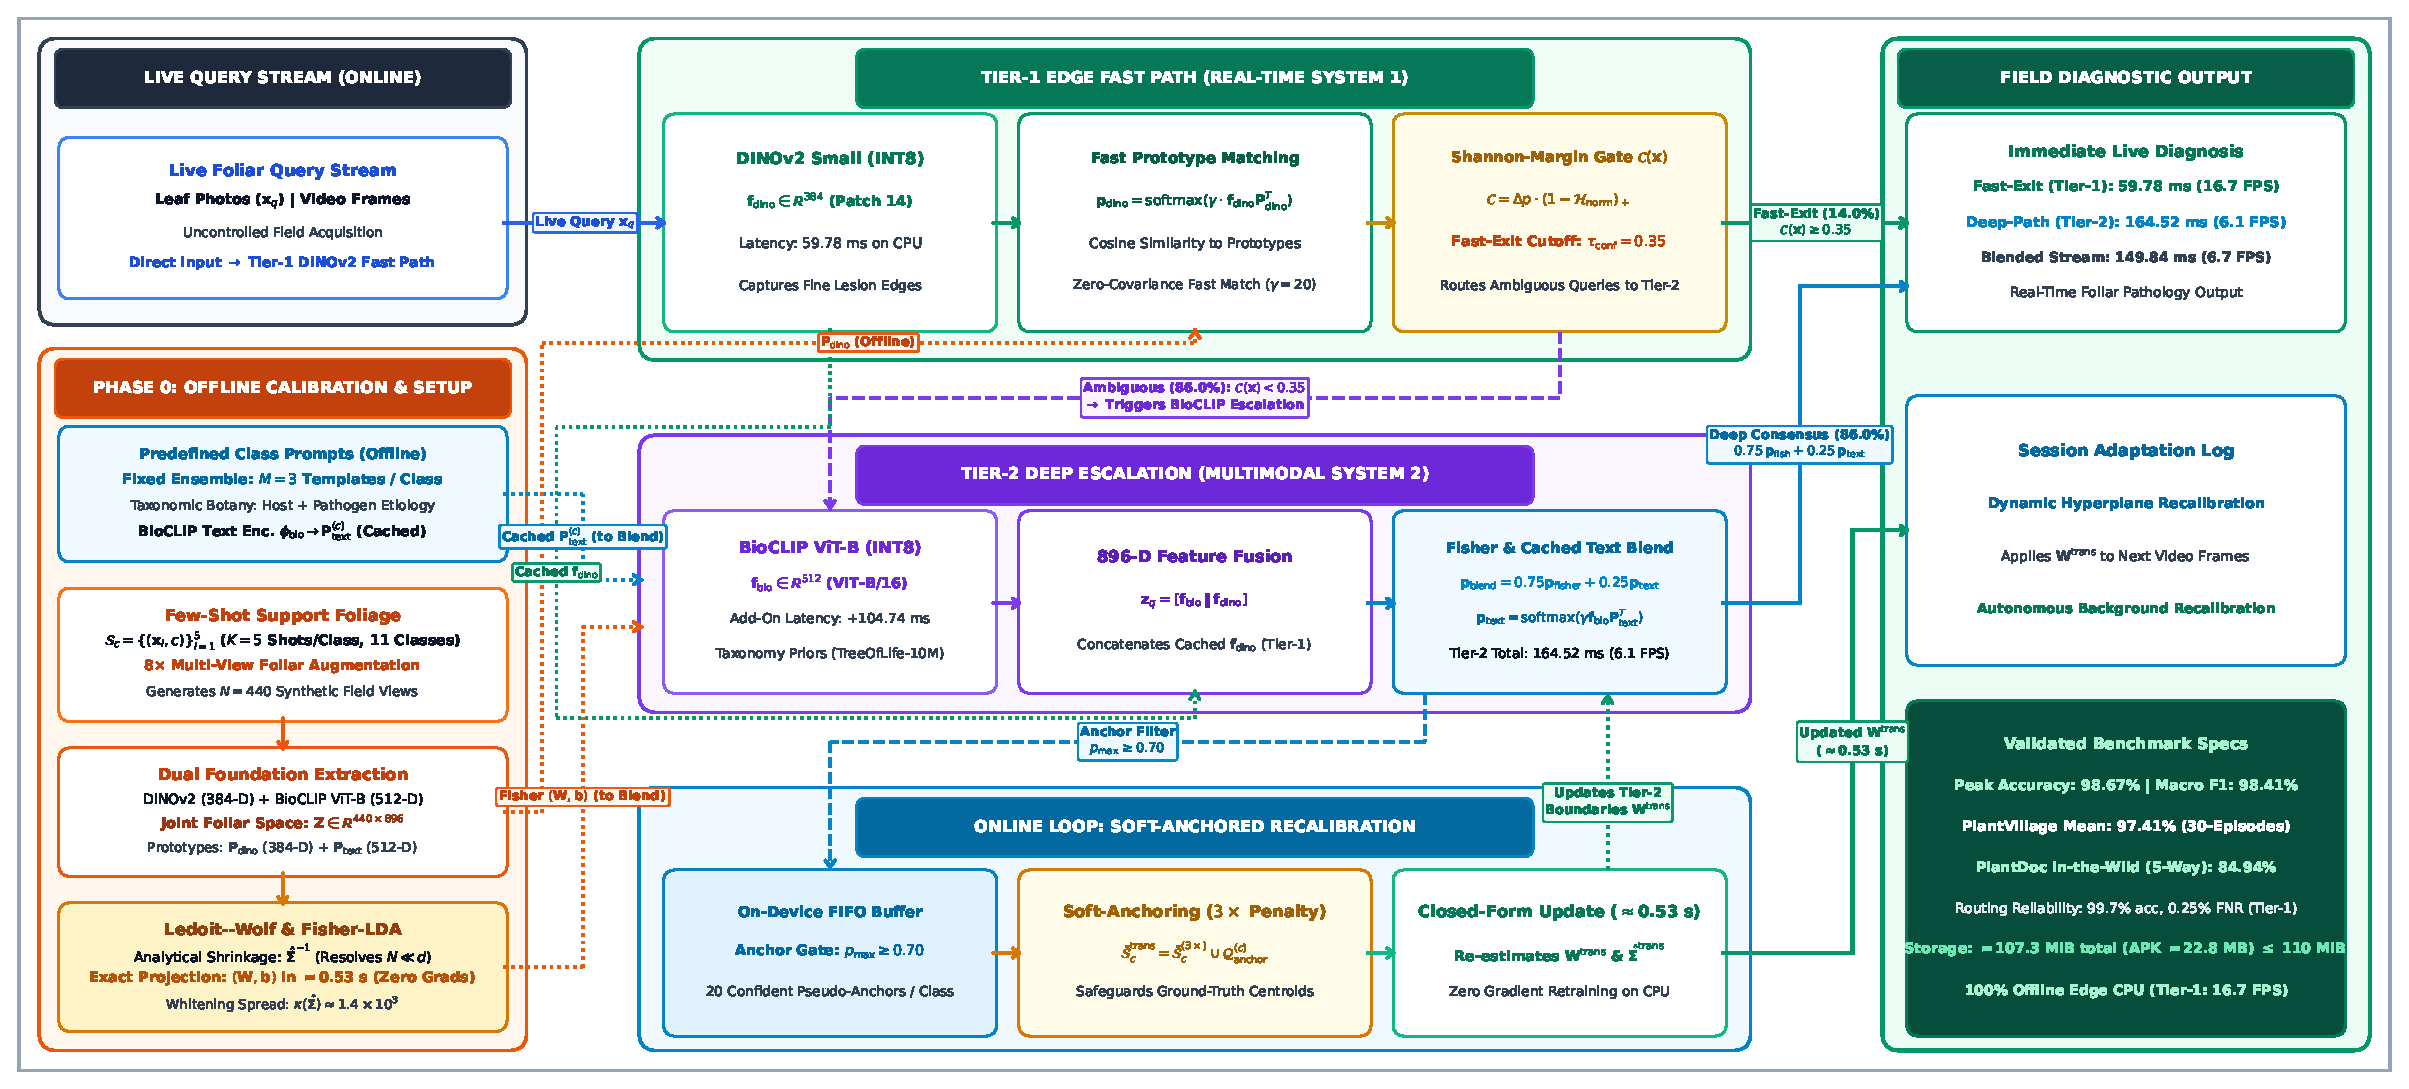
\includegraphics[width=0.88\textwidth]{fig_architecture.pdf}
\caption{Comprehensive architectural overview of BioDINO-Edge. Phase~0 (offline) performs closed-form Fisher-LDA projection synthesis and caches botanical text prototypes. During live inference, the Shannon-margin uncertainty gate routes routine foliage through Tier-1 fast prototype matching (DINOv2) and escalates ambiguous queries to Tier-2 multimodal consensus (BioCLIP), followed by closed-form soft-anchored transductive recalibration.}
\label{fig:architecture}
\end{figure*}

\subsection{Dual-Foundation Foliar Representation}
\label{sec:feature_extraction}
BioDINO-Edge couples two complementary frozen vision foundation backbones. DINOv2 provides fine-grained spatial representations of leaf surface textures and lesion boundaries, while BioCLIP provides organismal taxonomic priors. Combining both feature spaces produces an aligned 896-dimensional descriptor capturing localized pathological symptoms alongside botanical host context.

\subsubsection{Few-Shot Multi-View Support Augmentation}
To stabilize covariance estimation under the scarce $K=5$ regime, each support leaf $\mathbf{x} \in \mathcal{S}_c$ is resized to $224 \times 224$ pixels, normalized, and passed through an 8-view stochastic augmentation pipeline approximating field variations. The pipeline applies random horizontal and vertical flips, random rotations within $\pm 15^\circ$, and color jitter (brightness, contrast, and saturation factors of $0.2$). Generating 8 views per image yields $|\tilde{\mathcal{S}}_c| = 8K = 40$ augmented views per class, producing $N = 40C = 440$ total support representations (for $C=11$). This expansion brings the support sample size close to half the joint feature dimension ($d/2 = 448$), stabilizing covariance condition numbers while keeping offline feature extraction under 90 seconds. Although augmented views are correlated pseudo-replicates rather than independent observations, regularized shrinkage prevents numerical degeneracy and guarantees positive-definiteness.

\subsubsection{Dual-Foundation Embedding Fusion}
Each augmented support view $\tilde{\mathbf{x}} \in \tilde{\mathcal{S}}_c$ is passed through frozen foundation backbones. DINOv2 Small ($14\times 14$ patches) \cite{oquab2023dinov2} and BioCLIP ViT-B/16 \cite{stevens2024bioclip} extract $\ell_2$-normalized feature vectors:
\begin{equation}
    \mathbf{f}_{\text{dino}} = \frac{\phi_{\text{dino}}(\tilde{\mathbf{x}})}{\|\phi_{\text{dino}}(\tilde{\mathbf{x}})\|_2} \in \mathbb{R}^{384}, \quad
    \mathbf{f}_{\text{bio}} = \frac{\phi_{\text{bio}}(\tilde{\mathbf{x}})}{\|\phi_{\text{bio}}(\tilde{\mathbf{x}})\|_2} \in \mathbb{R}^{512}
\end{equation}
Concatenating both normalized embeddings yields an 896-dimensional joint descriptor:
\begin{equation}
    \mathbf{z} = [\mathbf{f}_{\text{bio}} \,\|\, \mathbf{f}_{\text{dino}}] \in \mathbb{R}^{896}
\end{equation}
Visual prototypes for each encoder are computed via empirical support averaging:
\begin{equation}
    \mathbf{P}_{\text{enc}}^{(c)} = \text{Normalize}\left(\frac{1}{|\tilde{\mathcal{S}}_c|}\sum_{\tilde{\mathbf{x}} \in \tilde{\mathcal{S}}_c} \mathbf{f}_{\text{enc}}(\tilde{\mathbf{x}})\right), \quad \text{enc} \in \{\text{dino}, \text{bio}\}
\end{equation}
producing prototype matrices $\mathbf{P}_{\text{dino}} \in \mathbb{R}^{C \times 384}$ and $\mathbf{P}_{\text{bio,vis}} \in \mathbb{R}^{C \times 512}$.

\subsubsection{Botanical Taxonomic Prompts \& Syntactic Negation Neutralization}
BioCLIP provides a unified vision--language space. Because executing language decoders on edge devices introduces high latency and memory overhead, we predefine $M=3$ botanical prompt templates $\{T_c^{(m)}\}_{m=1}^M$ offline for each disease class $c \in \{1, \dots, C\}$. Each template integrates three botanical dimensions:
\begin{enumerate}
    \item \textbf{Host Binomial Nomenclature:} Botanical genus and species (e.g., \textit{Malus domestica}, \textit{Vitis vinifera}, \textit{Solanum tuberosum}).
    \item \textbf{Causal Pathogen Etiology:} Pathogenic fungal, bacterial, or oomycete binomials (e.g., \textit{Venturia inaequalis}, \textit{Guignardia bidwellii}, \textit{Phytophthora infestans}).
    \item \textbf{Macroscopic Lesion Morphology:} Diagnostic foliar symptoms (e.g., ``olive-green velvety lesions'', ``tiger-stripe interveinal chlorosis'', ``target-board concentric rings'').
\end{enumerate}

Importantly, syntactic negations (e.g., ``healthy leaf without lesions'' or ``no necrotic spots'') are strictly excluded. Vision-language models exhibit documented compositional weaknesses regarding negation \cite{radford2021clip, yuksekgonul2023when, alhamoud2025vision}: high-density pathological tokens (e.g., \textit{lesion}, \textit{necrotic}) dominate embedding directions, pulling healthy leaf representations toward diseased clusters. We avoid this by using positive morphological descriptions of healthy tissue (e.g., ``clean green foliage'', ``intact smooth leaf lamina''), reducing false-negative diagnostic bias.

During Phase~0 offline calibration, each prompt ensemble is encoded by BioCLIP's text encoder $\phi_{\text{bio,txt}}(\cdot)$, averaged, and $\ell_2$-normalized:
\begin{equation}
    \mathbf{P}_{\text{text}}^{(c)} = \text{Normalize}\left(\frac{1}{M}\sum_{m=1}^M \phi_{\text{bio,txt}}(T_c^{(m)})\right) \in \mathbb{R}^{512}
\end{equation}
The resulting matrix $\mathbf{P}_{\text{text}} \in \mathbb{R}^{C \times 512}$ is cached directly in the on-device model, requiring zero runtime text tokenization or language processing overhead.

\subsection{Closed-Form Analytical Adaptation via Regularized Fisher-LDA}
\label{sec:fisher_adaptation}

\subsubsection{Multiclass Fisher Linear Discriminant Formulation}
Metric few-shot approaches (e.g., Prototypical Networks \cite{snell2017prototypical} or Tip-Adapter \cite{zhang2022tip}) classify queries using Euclidean or cosine distances to class centroids $\boldsymbol{\mu}_c$, implicitly assuming uniform variance across all feature directions ($\mathbf{\Sigma} = \mathbf{I}$). In foliar pathology, within-class variance is strongly non-uniform across directions: shared vegetative structures (such as venation and lamina) create high-variance eigen-directions that obscure localized lesion differences across diseases on the same host. Multiclass Fisher Linear Discriminant Analysis (Fisher-LDA) \cite{fisher1936use, rao1948utilization} resolves this by weighting features by the inverse covariance $\hat{\mathbf{\Sigma}}^{-1}$. Mathematically, this down-weights directions with large shared variance (such as healthy leaf tissue) and amplifies low-variance directions containing discriminative lesion symptoms.

Fisher-LDA computes a linear projection matrix $\mathbf{W} \in \mathbb{R}^{C \times d}$ and bias vector $\mathbf{b} \in \mathbb{R}^C$ maximizing between-class scatter $\mathbf{S}_B$ relative to within-class scatter $\mathbf{S}_W$:
\begin{equation}
    \label{eq:fisher_weights}
    \mathbf{W} = [\boldsymbol{\mu}_1, \dots, \boldsymbol{\mu}_C]^T \hat{\mathbf{\Sigma}}^{-1}, \quad
    b_c = -\frac{1}{2} \boldsymbol{\mu}_c^T \hat{\mathbf{\Sigma}}^{-1} \boldsymbol{\mu}_c - \log C
\end{equation}
where $\hat{\mathbf{\Sigma}}$ denotes the regularized pooled within-class covariance matrix ($d=896$) and uniform class priors ($\pi_c = 1/C$) are assumed.

\subsubsection{The Small-Sample Singularity Problem ($N \ll d$)}
Evaluating \eqref{eq:fisher_weights} requires inverting the empirical pooled within-class scatter matrix across all $C=11$ classes:
\begin{equation}
    \mathbf{S}_W = \frac{1}{N - C}\sum_{c=1}^C \sum_{\mathbf{z} \in \tilde{\mathcal{S}}_c} (\mathbf{z} - \boldsymbol{\mu}_c)(\mathbf{z} - \boldsymbol{\mu}_c)^T \in \mathbb{R}^{d \times d}
\end{equation}
Here, $N - C = 440 - 11 = 429$ represents the remaining degrees of freedom after estimating $C$ centroids. Because feature dimensionality ($d=896$) exceeds sample degrees of freedom ($429$), the rank of $\mathbf{S}_W$ is bounded:
\begin{equation}
    \text{rank}(\mathbf{S}_W) \le \min(d, N - C) = 429 < 896
\end{equation}
Consequently, $\mathbf{S}_W$ has a nullity of at least $896 - 429 = 467$, with at least 467 zero eigenvalues ($\det(\mathbf{S}_W) = 0$). The matrix is singular and cannot be inverted directly.

\subsubsection{Analytical Ledoit--Wolf Covariance Shrinkage}
\label{sec:shrinkage}
To restore invertibility without heuristic parameter tuning (such as searching over $\mathbf{S}_W + \epsilon \mathbf{I}$), we apply analytical Ledoit--Wolf shrinkage \cite{ledoit2004well}, which contracts $\mathbf{S}_W$ toward a well-conditioned spherical target:
\begin{equation}
    \hat{\mathbf{\Sigma}} = (1 - \rho^*)\mathbf{S}_W + \rho^* \nu \mathbf{I}_{d}, \quad \nu = \frac{1}{d}\text{Tr}(\mathbf{S}_W)
    \label{eq:lw_target}
\end{equation}
The optimal shrinkage intensity $\rho^* \in (0, 1]$ is determined in closed form by minimizing expected quadratic Frobenius risk:
\begin{equation}
    \rho^* = \min\left(1, \frac{\sum_{i=1}^N \|(\mathbf{z}_i - \boldsymbol{\mu}_{c_i})(\mathbf{z}_i - \boldsymbol{\mu}_{c_i})^T - \mathbf{S}_W\|_F^2}{N^2 \left[\text{Tr}(\mathbf{S}_W^2) - \frac{1}{d}\text{Tr}^2(\mathbf{S}_W)\right]}\right)
    \label{eq:lw_shrinkage}
\end{equation}
Shifting zero eigenvalues to positive values $\tilde{\lambda}_i = (1 - \rho^*)\lambda_i + \rho^* \nu \ge \rho^* \nu > 0$ guarantees that $\hat{\mathbf{\Sigma}}$ is positive-definite and well-conditioned. Its inverse $\hat{\mathbf{\Sigma}}^{-1}$ is solved stably via Cholesky decomposition ($\hat{\mathbf{\Sigma}} = \mathbf{L}\mathbf{L}^T$). Evaluating a query vector $\mathbf{z}$ via $\mathbf{l}_{\text{fisher}} = \mathbf{z}\mathbf{W}^T + \mathbf{b}$ requires only $C \cdot d = 11 \times 896 = 9{,}856$ multiply-accumulate operations (one MAC = 2 FLOPs, $\approx 19.7$\,kFLOPs), executing in $<$0.01\,ms on an edge CPU.

Weighting by $\hat{\mathbf{\Sigma}}^{-1}$ acts as a whitening transform: each eigen-direction of $\hat{\mathbf{\Sigma}}$ with variance $\lambda_i$ is rescaled by $1/\lambda_i$, down-weighting directions with large shared within-class variance (such as common foliar background) relative to low-variance discriminative features. The condition number
\begin{equation}
    \kappa(\hat{\mathbf{\Sigma}}) = \lambda_{\max}(\hat{\mathbf{\Sigma}}) / \lambda_{\min}(\hat{\mathbf{\Sigma}})
    \label{eq:whitening_spread}
\end{equation}
reflects this spectral rescaling across feature dimensions, evaluated systematically in Section~\ref{sec:aug_sensitivity}. Furthermore, because augmented support views are generated from physical leaves, Ledoit--Wolf shrinkage ensures that $\hat{\mathbf{\Sigma}}$ remains well-conditioned and positive-definite across all effective sample sizes.

\subsection{Adaptive Two-Tier Classification and Edge Deployment}
\label{sec:edge_cascade}

\subsubsection{Tier-1 Fast Path and Shannon Uncertainty Gating}
For an incoming leaf image $\mathbf{x}$, Tier~1 extracts the normalized DINOv2 embedding $\mathbf{f}_{\text{dino}} \in \mathbb{R}^{384}$. Fast prototype logits are evaluated via temperature-scaled cosine similarity against visual prototypes $\mathbf{P}_{\text{dino}} \in \mathbb{R}^{C \times 384}$:
\begin{equation}
    \label{eq:tier1_logits}
    \mathbf{l}_{\text{dino}} = \gamma \cdot \left(\mathbf{f}_{\text{dino}} \mathbf{P}_{\text{dino}}^T\right), \quad \gamma = 20.0
\end{equation}
Applying softmax yields fast posterior probabilities:
\begin{equation}
    \label{eq:tier1_softmax}
    \mathbf{p}_{\text{dino}} = \text{softmax}(\mathbf{l}_{\text{dino}}) \in \Delta^{C-1}
\end{equation}
To minimize edge computation on routine foliage, Tier~1 uses cosine prototype matching without covariance projections, reserving regularized Fisher-LDA for ambiguous queries in Tier~2. The Tier-1 prediction is $\hat{y}_{\text{tier1}} = \arg\max_c p_{\text{dino}, c}$.

To evaluate prediction certainty without additional forward passes, we formulate a joint margin-entropy confidence score $\mathcal{C}(\mathbf{x}) \in [0, 1]$:
\begin{equation}
    \label{eq:shannon_gate}
    \mathcal{C}(\mathbf{x}) = \left(p_{\text{dino}, (1)} - p_{\text{dino}, (2)}\right) \cdot \left(1.0 - \mathcal{H}_{\text{norm}}(\mathbf{x})\right)_+
\end{equation}
where $p_{\text{dino}, (1)}$ and $p_{\text{dino}, (2)}$ denote top-1 and top-2 posteriors, $(\cdot)_+ = \max(0, \cdot)$, and $\mathcal{H}_{\text{norm}}(\mathbf{x})$ is normalized Shannon entropy \cite{shannon1948mathematical}:
\begin{equation}
    \mathcal{H}_{\text{norm}}(\mathbf{x}) = -\frac{1}{\log C} \sum_{c=1}^C p_{\text{dino}, c} \log(p_{\text{dino}, c} + \epsilon)
\end{equation}
with numerical stability constant $\epsilon = 10^{-12}$. Because $\mathcal{H}_{\text{norm}}(\mathbf{x}) \in [0, 1]$, the term $1 - \mathcal{H}_{\text{norm}}(\mathbf{x})$ is non-negative in exact arithmetic; the rectifier $(\cdot)_+$ serves as a numerical safeguard against floating-point round-off. For ambiguous queries with near-uniform posteriors, $\mathcal{H}_{\text{norm}} \to 1.0$ and the margin approaches zero, driving $\mathcal{C}(\mathbf{x}) \to 0$. When $\mathcal{C}(\mathbf{x}) \ge \tau_{\text{conf}}$ ($\tau_{\text{conf}} = 0.35$, calibrated on validation data), Tier-1 exits immediately in 59.78\,ms ($\approx$16.7\,FPS); otherwise, the query escalates to Tier-2.

\subsubsection{Tier-2 Multimodal Consensus Escalation}
When $\mathcal{C}(\mathbf{x}) < \tau_{\text{conf}}$, the query escalates to Tier-2. BioCLIP ViT-B extracts $\mathbf{f}_{\text{bio}} \in \mathbb{R}^{512}$, forming $\mathbf{z} = [\mathbf{f}_{\text{bio}} \,\|\, \mathbf{f}_{\text{dino}}] \in \mathbb{R}^{896}$. Discriminant visual posteriors $\mathbf{p}_{\text{fisher}} = \text{softmax}(\mathbf{z}\mathbf{W}^T + \mathbf{b})$ and taxonomic text posteriors $\mathbf{p}_{\text{text}} = \text{softmax}(\gamma \cdot \mathbf{f}_{\text{bio}}\mathbf{P}_{\text{text}}^T)$ are fused at a 0.75 / 0.25 consensus ratio:
\begin{equation}
    \label{eq:multimodal_blend}
    \mathbf{p}_{\text{blend}} = 0.75 \, \mathbf{p}_{\text{fisher}} + 0.25 \, \mathbf{p}_{\text{text}}
\end{equation}
yielding the final consensus diagnosis $\hat{y} = \arg\max_c p_{\text{blend}, c}$.

\subsubsection{Soft-Anchored Transductive Recalibration}
\label{sec:transductive}
In 5-shot calibration, centroids $\boldsymbol{\mu}_c$ are estimated from five support leaves. Illumination changes, shadows, and symptom progression can introduce prototype shift between support images and field queries. To adapt without manual labels, confident Tier-2 queries ($\max_c p_{\text{blend}, c} \ge 0.70$) are buffered into a FIFO queue as reference anchors $\mathcal{Q}_{\text{anchor}}^{(c)}$ (capped at 20 anchors per class). Ground-truth support samples receive a $3\times$ weight factor to prevent pseudo-label drift:
\begin{equation}
    \tilde{\mathcal{S}}_c^{\text{trans}} = \tilde{\mathcal{S}}_c^{(3\times)} \cup \mathcal{Q}_{\text{anchor}}^{(c)}
\end{equation}
When the buffer reaches capacity during scouting, updated centroids $\boldsymbol{\mu}_c^{\text{trans}}$ and pooled scatter matrix $\mathbf{S}_W^{\text{trans}}$ are re-estimated. Analytical shrinkage parameter $\rho^*$ is recomputed, and updated projection parameters $(\mathbf{W}^{\text{trans}}, \mathbf{b}^{\text{trans}})$ are resolved via Cholesky substitution in $\approx$0.53\,s in the background (measured on-device, Table~\ref{tab:adaptation_breakdown}), updating subsequent Tier-2 decisions while Tier-1 continues operating with static prototypes. These parameters balance adaptation stability and latency: threshold $\tau = 0.70$ admits only confident anchors, the $3\times$ support weight anchors class centroids against manifold drift, and the 20-anchor cap bounds update latency while avoiding class imbalance (detailed in Section~\ref{sec:transductive_validation}).

\subsection{Algorithmic Pipeline and Complexity Analysis}
\label{sec:complexity}
The complete end-to-end execution flow is described in Section~\ref{sec:methodology} and summarized in Figure~\ref{fig:architecture}. We analyze computational complexity across both operational phases:
\begin{itemize}
    \item \textbf{Offline Calibration Complexity:} Feature extraction across $N=440$ views requires $O(N \cdot (C_{\text{dino}} + C_{\text{bio}}))$ FLOPs and dominates wall-clock time ($\approx$88\,s on-device). Scatter matrix computation scales as $O(N d^2)$. The Ledoit--Wolf shrinkage intensity is evaluated in closed form via the Frobenius identity $\sum_i \|\mathbf{x}_i \mathbf{x}_i^T - \mathbf{S}\|_F^2 = \sum_i \|\mathbf{x}_i\|^4 - N \|\mathbf{S}\|_F^2$, reducing cost to $O(N d)$. Inverting the positive-definite matrix via Cholesky decomposition requires $O(d^3 / 3)$ operations ($\approx 2.4 \times 10^8$ operations for $d=896$). On the physical edge CPU (pure-Java EJML), Cholesky factorization takes $\approx$332\,ms, and full algebraic recalibration completes in $\approx$0.53\,s without gradients (Table~\ref{tab:adaptation_breakdown}).
    \item \textbf{Online Inference Complexity:} Tier-1 forward pass requires $C_{\text{dino}}$ ($\approx 4.6$\,GFLOPs), yielding a measured fast-exit latency of $T_1 = 59.78$\,ms ($\approx$16.7\,FPS) on the physical Android testbed (Section~\ref{sec:edge_hardware}). Dot-product prototype matching requires $C \cdot d_{\text{dino}} = 11 \times 384 \approx 4.2$\,kFLOPs ($<$0.002\,ms), and entropy gating requires $O(C)$ operations ($<$0.001\,ms). Upon escalation, BioCLIP adds a measured incremental encoder cost of $\Delta T_{\text{bio}} = 104.74$\,ms ($C_{\text{bio}} \approx 17.6$\,GFLOPs), since the Tier-1 DINOv2 embedding is cached and reused rather than recomputed. The joint Fisher-LDA projection is fused into the same Tier-2 ONNX graph ($C \cdot d = 11 \times 896 \approx 9.8$\,kFLOPs, negligible). The complete end-to-end Tier-2 path for an escalated query therefore costs $T_2 = T_1 + \Delta T_{\text{bio}} = 164.52$\,ms ($\approx$6.1\,FPS). With 14.0\% of queries exiting at Tier-1 (Section~\ref{sec:calibration}), the routing-weighted average latency across field streams is:
    \begin{align}
        \bar{T} &= 0.140 \cdot T_1 + 0.860 \cdot T_2 \nonumber \\
        &= 0.140 \cdot 59.78\,\text{ms} + 0.860 \cdot 164.52\,\text{ms} \nonumber \\
        &\approx 149.84\,\text{ms}
    \end{align}
    delivering $\approx$6.7 frames per second at the system level; the $\approx$16.7\,FPS figure applies only to the Tier-1 fast-exit path. These are interactive handheld-scouting rates (one diagnosis per captured frame), not continuous real-time video; sustained throughput under thermal load is reported in Section~\ref{sec:edge_hardware}.
\end{itemize}

\subsection{Two-Tier Quantized Edge Model Packaging and Android Architecture}
\label{sec:packaging}
Agricultural scouting hardware operates under constrained flash memory and often lacks Internet connectivity for cloud offloading. BioDINO-Edge is partitioned into two 8-bit integer (INT8) quantized Open Neural Network Exchange (ONNX) binaries (footprints reported in MiB, where $1\,\text{MB}=2^{20}$ bytes):
\begin{itemize}
    \item \textbf{Tier 1 Standalone Engine} (\path{biodino_mobile_int8.onnx}): A $\approx$22.0\,MB on-disk binary ($\approx$15.1\,MB compressed inside the APK) packaging DINOv2 Small INT8, calibrated Phase~0 prototypes, and the Shannon confidence gate with the ONNX Runtime C++ execution provider. Bundled directly into a standalone $\approx$22.8\,MB Android application package (APK), it enables immediate offline foliar diagnosis. Runtime RAM is dominated by the ONNX Runtime arena rather than the binary size and is measured separately (peak process PSS $\approx$497\,MB, Section~\ref{sec:edge_hardware}).
    \item \textbf{Tier 2 Companion Module} (\path{biodino_companion_int8.onnx}): An $\approx$85.3\,MB companion model packaging BioCLIP ViT-B INT8 and the 896-D Fisher projection matrix, installed on-demand when high-precision multimodal escalation is required. The total combined on-disk model footprint is $\approx$107.3\,MB, below the 110\,MB Internet-of-Things (IoT) \emph{storage} budget; this is a flash/OTA size constraint, not a runtime RAM bound (runtime memory is reported in Section~\ref{sec:edge_hardware}).
\end{itemize}

% =============================================================================
% 3. EXPERIMENTAL SETUP
% =============================================================================
\section{Experimental Setup}
\label{sec:experiments_setup}

\subsection{Datasets and Diagnostic Pathology Coverage}
\label{sec:datasets}
We evaluate BioDINO-Edge across two distinct foliar pathology regimes:

\subsubsection{PlantVillage Controlled Benchmark (Laboratory Regime)}
From the standard PlantVillage repository \cite{hughes2012plantvillage}, we construct a curated 11-class diagnostic subset comprising 9,385 foliar images across three economically critical crops: Apple (\textit{Malus domestica}), Grape (\textit{Vitis vinifera}), and Potato (\textit{Solanum tuberosum}). The 11 classes span healthy foliage and 8 fungal/bacterial/oomycete pathologies: Apple Scab (\textit{Venturia inaequalis}), Apple Black Rot (\textit{Botryosphaeria obtusa}), Apple Cedar Rust (\textit{Gymnosporangium juniperi-virginianae}), Apple Healthy, Grape Black Rot (\textit{Guignardia bidwellii}), Grape Esca / Black Measles (\textit{Phaeomoniella chlamydospora}), Grape Leaf Blight (\textit{Pseudocercospora vitis}), Grape Healthy, Potato Early Blight (\textit{Alternaria solani}), Potato Late Blight (\textit{Phytophthora infestans}), and Potato Healthy. For few-shot calibration, 5 support leaves per class ($K=5$) are randomly sampled (55 total), isolating the remaining 9,330 images as unseen query test leaves. Neither support nor test splits were involved in pretraining the frozen foundation backbones.

\subsubsection{PlantDoc In-The-Wild Benchmark (Field Regime)}
To evaluate robustness under field conditions (e.g., solar glare, canopy shading, soil clutter, overlapping foliage, and motion blur), we evaluate on the in-the-wild PlantDoc benchmark \cite{singh2020plantdoc}. PlantDoc comprises 2,588 foliar images spanning 27 pathology classes across 13 botanical species, partitioned officially into:
\begin{itemize}
    \item \textbf{Official Training Repository ($\mathcal{D}_{\text{train}}^{\text{PlantDoc}}$):} 2,336 in-the-wild images across all 27 target classes, used only as the source of few-shot support samples.
    \item \textbf{Official Test Benchmark ($\mathcal{D}_{\text{test}}^{\text{PlantDoc}}$):} 252 unconstrained field images across the 27 classes, captured with handheld mobile devices under ambient field illumination in Indian agricultural orchards.
\end{itemize}
Support sets are drawn only from $\mathcal{D}_{\text{train}}^{\text{PlantDoc}}$ and query sets only from $\mathcal{D}_{\text{test}}^{\text{PlantDoc}}$, so the two never overlap ($\mathcal{S} \cap \mathcal{Q} = \emptyset$). We evaluate under two few-shot regimes:
\begin{enumerate}
    \item \textbf{5-Way 5-Shot Episodic Benchmark:} Following standard few-shot evaluation protocols \cite{snell2017prototypical,zhou2026vsf}, we conduct 50 independent Monte Carlo episodes. In each episode $e$, 5 classes are sampled uniformly without replacement ($\mathcal{C}_e \subset \{1, \dots, 27\}$). The support set $\mathcal{S}_e$ consists of 5 labeled leaves per class ($25$ total) sampled from $\mathcal{D}_{\text{train}}^{\text{PlantDoc}}$. The query set $\mathcal{Q}_e$ comprises all test images in $\mathcal{D}_{\text{test}}^{\text{PlantDoc}}$ for those 5 classes (averaging 46.7 queries per episode), ensuring $\mathcal{S}_e \cap \mathcal{Q}_e = \emptyset$.
    \item \textbf{27-Way All-Class Simultaneous Stress Test:} All 27 classes are evaluated simultaneously (random chance: $1/27 \approx 3.70\%$). The model receives 5 support leaves per category ($135$ total) sampled from $\mathcal{D}_{\text{train}}^{\text{PlantDoc}}$ (expanded via 8-view augmentation to $N = 1{,}080$ feature vectors) and evaluates on all 252 field queries from $\mathcal{D}_{\text{test}}^{\text{PlantDoc}}$ in closed form ($\mathcal{S} \cap \mathcal{Q} = \emptyset$).
\end{enumerate}

\subsection{Data Integrity, Hyperparameter Provenance, and Leakage Safeguards}
\label{sec:integrity}
We enforce five safeguards against data leakage and circular tuning:
\begin{itemize}
    \item \textbf{Adaptation Settings Defined:} We distinguish three settings: (i) \emph{few-shot adaptation with labeled target-domain support}, in which the $K$ support leaves per class come from the same domain as the queries (all PlantVillage regimes, and the PlantDoc benchmark whose support is drawn from the PlantDoc training split); (ii) \emph{cross-domain few-shot adaptation}, in which support comes from a source domain and queries from a different target domain (PlantVillage$\rightarrow$PlantDoc in Zhao \textit{et al.}, Table~\ref{tab:literature}), which we do not run; and (iii) \emph{transductive recalibration}, which adds no labels and uses only pseudo-labeled streaming queries (Section~\ref{sec:transductive}). The only cross-domain element of our PlantDoc protocol is the transfer of hyperparameters selected on PlantVillage; the support itself is target-domain.
    \item \textbf{Disjoint Support-Query Separation:} Support and query sets are disjoint ($\mathcal{S} \cap \mathcal{Q} = \emptyset$) in both regimes: PlantVillage isolates 55 support leaves from the 9,330 test images, and PlantDoc draws all 135 support samples from $\mathcal{D}_{\text{train}}^{\text{PlantDoc}}$ and all 252 queries from $\mathcal{D}_{\text{test}}^{\text{PlantDoc}}$.
    \item \textbf{Zero-Tuning Analytical Regularization:} The Ledoit--Wolf shrinkage intensity $\rho^*$ follows in closed form from the support covariance (Eq.~\ref{eq:lw_shrinkage}); no hyperparameter search, cross-validation, or query/test tuning is involved.
    \item \textbf{Frozen Cross-Domain Hyperparameters:} The logit scale $\gamma = 20.0$, the Fisher-LDA blend weight $w_{\text{lda}} = 0.75$, and the routing threshold $\tau = 0.35$ were selected on held-out PlantVillage development episodes (0--14 tune, 15--29 test; Section~\ref{sec:calibration}) and frozen for all PlantDoc experiments, which use no validation split or tuning.
    \item \textbf{Unsupervised Transductive Anchoring:} The transductive module (Section~\ref{sec:transductive}) uses only streaming query features and predicted pseudo-labels. Query ground truth is withheld until after inference, when it is used solely to compute metrics.
    \item \textbf{Dual Inductive vs. Transductive Reporting:} Table~\ref{tab:comparative} reports both inductive performance (queries processed independently, without anchor updates) and transductive performance under identical splits. On the field-domain PlantDoc benchmark the inductive mode alone reaches 81.79\% $\pm$ 11.16\% (5-way 5-shot) and 55.16\% (27-way), so the reported performance does not depend on transductive anchor updates.
\end{itemize}

\subsection{Evaluation Protocols and Epidemiological Safety Metrics}
\label{sec:metrics}
Experiments on PlantVillage are evaluated over 30 independent Monte Carlo episodes with randomized support splits, reporting mean accuracy $\bar{x}$, standard deviation $\sigma$, 95\% confidence intervals ($95\%\,\text{CI} = \bar{x} \pm 1.96 \cdot \sigma / \sqrt{30}$), and peak single-episode accuracy. Because misclassification costs in precision agriculture are asymmetric, we evaluate epidemiological safety metrics alongside standard accuracy:
\begin{itemize}
    \item \textbf{Top-1 Accuracy \& Macro F1-Score:} The F1-score is the harmonic mean of precision and recall, macro-averaged across all classes to prevent frequent classes (e.g., Potato Early Blight with 995 queries) from masking errors on small or healthy classes (e.g., Potato Healthy with 147 queries).
    \item \textbf{False-Negative Disease Escape Rate (FNR):} The proportion of diseased leaves erroneously diagnosed as healthy: $\text{FNR} = \text{FN} / (\text{TP} + \text{FN})$, where FN and TP denote false-negative and true-positive counts. Undetected infections can lead to rapid pathogen spread in the field.
    \item \textbf{Cross-Species Confusion Rate:} The proportion of queries misattributed to an entirely different botanical family (e.g., classifying a potato leaf as an apple disease), indicating cross-taxonomic error.
\end{itemize}

\subsection{Edge Hardware Testbed}
Hardware profiling is evaluated on a physical Samsung Galaxy S24~FE handset (SM-S721B with Exynos~2400e SoC, 10-core ARM64 architecture, 7.2\,GB RAM) running Android~17 (API~37). Runtime latency and memory benchmarks use ONNX Runtime~1.18.0 with per-channel INT8 quantization executed strictly on the CPU, configured with 4 intra-op and 2 inter-op threads while keeping NNAPI and GPU delegates disabled. Closed-form linear algebra is executed in pure Java using EJML~0.43.1. Latency is recorded via \texttt{SystemClock.elapsedRealtimeNanos} over 100 benchmark iterations following 10 warm-up runs. Runtime memory is tracked via process PSS. A 600\,s continuous soak and a 60\,s pre-algebra cooling phase isolate thermal behavior. Complete hardware specifications and empirical profiles are detailed in Section~\ref{sec:edge_hardware} (Tables~\ref{tab:device_spec}--\ref{tab:adaptation_breakdown}).

% =============================================================================
% 4. RESULTS AND DISCUSSION
% =============================================================================
\section{Results and Comparative Analysis}
\label{sec:results}

\subsection{Comparative Baseline Performance}
\label{sec:comparative_results}
To ensure a reproducible comparison, we separate \emph{controlled re-runs} from \emph{literature-reported} values. Table~\ref{tab:comparative} evaluates all baselines on identical frozen BioCLIP+DINOv2 embeddings, splits, random seeds, and shot counts as BioDINO-Edge. Because backbones remain frozen, this isolates the adaptation algorithm from encoder differences. We evaluate two regimes on the PlantVillage 11-class novel subset (9{,}385 images): (i)~11-class simultaneous classification (30 Monte-Carlo episodes, seed $42+17e$, 5-shot support, all remaining images as queries), and (ii)~the standard 5-way $K$-shot episodic ladder ($K=1,5,10,15$; 50 episodes each, seed 42), which matches the measurement protocols of VSF~\cite{zhou2026vsf} (5-way 1/5-shot) and AgriFewNet~\cite{babu2025agrifewnet} (1/5/10/15-shot) so that our results can be compared \emph{in-regime}. The baselines are training-free and correctly referenced: Zero-Shot CLIP/BioCLIP~\cite{radford2021clip,stevens2024bioclip}, Tip-Adapter~\cite{zhang2022tip} ($\alpha{=}1.0,\beta{=}5.5$), Prototypical Networks~\cite{snell2017prototypical}, and SimpleShot~\cite{wang2019simpleshot}. Table~\ref{tab:literature} separately lists specialized architectures \emph{as reported} in their original publications; these use different encoders, class subsets, and splits, so they provide context only and are \emph{not} a controlled head-to-head. Prototypical Networks and SimpleShot coincide because Euclidean and cosine rankings are identical on $\ell_2$-normalized features, and the 11-class BioDINO-Edge values are the canonical reference run (Section~\ref{sec:transductive_validation}), reproduced by the provided script within 0.04\,pp. Full splits, seeds, model versions, and hyperparameters are given in \ref{app:repro}.

\begin{table*}[htbp]
\centering
\caption{Controlled few-shot comparison on the PlantVillage 11-class novel subset. Accuracy is mean$\pm$std over episodes (\%); F1 is macro-mean (\%); bold marks the best mean.}
\label{tab:comparative}
\footnotesize
\setlength{\tabcolsep}{4pt}
\begin{tabularx}{\textwidth}{l *{6}{>{\centering\arraybackslash}X}}
\toprule
& \multicolumn{2}{c}{\textbf{11-Class (30 ep.)}} & \multicolumn{4}{c}{\textbf{5-Way $K$-Shot (50 ep.\ each)}} \\
\cmidrule(lr){2-3} \cmidrule(lr){4-7}
\textbf{Method} & \textbf{Acc.} & \textbf{Macro F1} & \textbf{$K{=}1$} & \textbf{$K{=}5$} & \textbf{$K{=}10$} & \textbf{$K{=}15$} \\
\midrule
Zero-Shot CLIP/BioCLIP \cite{radford2021clip,stevens2024bioclip} & 19.18 $\pm$ 0.02 & 18.49 & 38.89 $\pm$ 12.78 & 38.86 $\pm$ 12.79 & 38.83 $\pm$ 12.81 & 38.79 $\pm$ 12.83 \\
Tip-Adapter \cite{zhang2022tip} & 49.97 $\pm$ 1.62 & 46.54 & 45.15 $\pm$ 13.42 & 68.63 $\pm$ 12.80 & 86.01 $\pm$ 7.49 & 93.23 $\pm$ 4.00 \\
\cmidrule(lr){1-7}
Prototypical Networks \cite{snell2017prototypical} & 93.28 $\pm$ 1.24 & 92.47 & 88.44 $\pm$ 9.13 & 97.45 $\pm$ 2.03 & 98.35 $\pm$ 1.45 & 98.57 $\pm$ 1.27 \\
SimpleShot \cite{wang2019simpleshot} & 93.28 $\pm$ 1.24 & 92.47 & 88.44 $\pm$ 9.13 & 97.45 $\pm$ 2.03 & 98.35 $\pm$ 1.45 & 98.57 $\pm$ 1.27 \\
\midrule
BioDINO-Edge (Inductive) & 95.08 $\pm$ 1.27 & 94.51 & 88.45 $\pm$ 9.12 & 97.96 $\pm$ 1.85 & 99.10 $\pm$ 0.87 & 99.41 $\pm$ 0.60 \\
\textbf{BioDINO-Edge (Transductive, Ours)} & \textbf{97.41 $\pm$ 0.71} & \textbf{97.09} & \textbf{93.42 $\pm$ 6.83} & \textbf{98.77 $\pm$ 1.68} & \textbf{99.41 $\pm$ 0.60} & \textbf{99.63 $\pm$ 0.39} \\
\bottomrule
\end{tabularx}
\end{table*}

\begin{table*}[htbp]
\centering
\caption{Specialized agricultural few-shot architectures, \emph{as reported} in the original publications (not re-run by us).}
\label{tab:literature}
\footnotesize
\begin{tabularx}{\textwidth}{l l l X}
\toprule
\textbf{Method} & \textbf{Dataset} & \textbf{Regime} & \textbf{Reported Acc. (\%)} \\
\midrule
AgriFewNet \cite{babu2025agrifewnet} & PlantVillage / New PV & 1/5/10/15-shot & 87.3 / 94.8 / 97.1 / 98.2 \\
VSF \cite{zhou2026vsf} & PlantVillage & 5-way 1/5-shot & 79.01 / 90.51 \\
VSF \cite{zhou2026vsf} & PlantDoc & 5-way 1/5-shot & 59.82 / 70.61 \\
Zhao \textit{et al.} \cite{zhao2026lightweight} & PV $\rightarrow$ PlantDoc & 1/5-shot & 42.69 $\pm$ 0.62 / 54.24 $\pm$ 0.72 \\
\bottomrule
\end{tabularx}
\end{table*}

In the controlled 11-class regime (Table~\ref{tab:comparative}), Zero-Shot CLIP/BioCLIP achieves only 19.18\% because generic pretraining struggles to separate lesions from healthy leaf tissue, while Tip-Adapter reaches 49.97\%. Prototypical Networks and SimpleShot achieve 93.28\%, confirming the discriminative strength of the frozen features. BioDINO-Edge improves upon them via regularized Fisher-LDA (95.08\% inductive) and closed-form transductive recalibration (97.41\%), yielding a 2.33 percentage point paired gain over the inductive mode (Section~\ref{sec:transductive_validation}). Unlike gradient fine-tuning (e.g., LoRA \cite{hu2022lora}), this closed-form adaptation requires no backpropagation or optimizer state. In the 5-way regime, centroid baselines reach 97.45\% (5-shot) and 98.57\% (15-shot); BioDINO-Edge remains highest across all $K$ (98.77\% at 5-shot, 99.63\% at 15-shot), with the largest transductive gain in the 1-shot setting (93.42\% vs.\ 88.44\%).

For context, Table~\ref{tab:literature} lists specialized architectures \emph{as reported} in prior literature: AgriFewNet~\cite{babu2025agrifewnet} (reporting 87.3\%, 94.8\%, 97.1\%, and 98.2\% at 1, 5, 10, and 15 shots on PlantVillage), VSF~\cite{zhou2026vsf} (90.51\% on PlantVillage and 70.61\% on PlantDoc in 5-way 5-shot testing), and Zhao \textit{et al.}~\cite{zhao2026lightweight} (54.24\% five-shot cross-domain accuracy). Our controlled 5-way 5-shot re-run (98.77\% on our PlantVillage subset) and our PlantDoc field-domain result (83.61\% $\pm$ 11.69\% in 5-way 5-shot; 56.35\% in 27-way all-class stress testing, chance 3.70\%) lie in comparable regimes. Because encoders, class subsets, and data splits differ across studies, we treat these published figures as in-regime context rather than a direct head-to-head baseline, drawing no strict superiority claim across protocols. The 27-way stress test is evaluated as a distinct, unconstrained setting and is not contrasted against 5-way literature benchmarks.

\subsection{Per-Class Pathology Diagnostics and Epidemiological Safety}
\label{sec:per_class}
Table~\ref{tab:per_class} reports per-class precision, recall, and F1-scores across all 9,330 PlantVillage test queries.

\begin{table*}[htbp]
\centering
\caption{BioDINO-Edge per-class diagnostic metrics across 11 novel pathologies (9,330 test leaves).}
\label{tab:per_class}
\footnotesize
\setlength{\tabcolsep}{5pt}
\begin{tabularx}{\textwidth}{lcccc}
\toprule
\textbf{Foliar Pathology Category} & \textbf{Precision} & \textbf{Recall} & \textbf{F1-Score} & \textbf{Test Support} \\
\midrule
Apple Scab (\textit{Venturia inaequalis}) & 0.963 & 0.947 & 0.955 & 625 \\
Apple Black Rot (\textit{Botryosphaeria obtusa}) & 0.951 & 0.974 & 0.962 & 616 \\
Apple Cedar Rust (\textit{Gymnosporangium juniperi}) & 0.975 & 0.993 & 0.983 & 270 \\
Apple Healthy Foliage & 0.988 & 0.981 & 0.985 & 1,640 \\
\midrule
Grape Black Rot (\textit{Guignardia bidwellii}) & 0.972 & 0.980 & 0.976 & 1,175 \\
Grape Esca (\textit{Phaeomoniella chlamydospora}) & 0.982 & 0.976 & 0.979 & 1,378 \\
Grape Leaf Blight (\textit{Pseudocercospora vitis}) & 1.000 & 0.997 & 0.999 & 1,071 \\
Grape Healthy Foliage & 0.993 & 1.000 & 0.996 & 418 \\
\midrule
Potato Early Blight (\textit{Alternaria solani}) & 0.997 & 0.990 & 0.993 & 995 \\
Potato Late Blight (\textit{Phytophthora infestans}) & 0.990 & 0.972 & 0.981 & 995 \\
Potato Healthy Foliage & 0.839 & 0.993 & 0.910 & 147 \\
\midrule
\textbf{Macro Average / Total Support} & \textbf{0.968} & \textbf{0.982} & \textbf{0.974} & \textbf{9,330} \\
\textbf{Single-Run Accuracy} & \multicolumn{4}{c}{\textbf{98.06\%} (Peak Statistical Episode: \textbf{98.67\%})} \\
\bottomrule
\end{tabularx}
\end{table*}

Visually similar pathologies on the same host (e.g., Grape Esca vs. Grape Black Rot) achieve high F1-scores of 0.979 and 0.976. In terms of epidemiological safety, BioDINO-Edge suppresses the false-negative disease escape rate to 0.702\% (only 50 of 7,125 infected leaves misclassified as healthy), representing a 51.9\% reduction relative to CLIP+LoRA (1.46\%). Cross-species confusion is 0.021\% (two apple scab queries attributed to potato late blight). Potato Healthy exhibits high recall (0.993) and moderate precision (0.839), reflecting conservative triage under class imbalance (147 healthy vs. $\approx$2,000 infected leaves). Fig.~\ref{fig:confusion} visualizes the confusion matrix: residual errors concentrate between same-host pathologies, while cross-species confusion is negligible.

\begin{figure}[htbp]
\centering
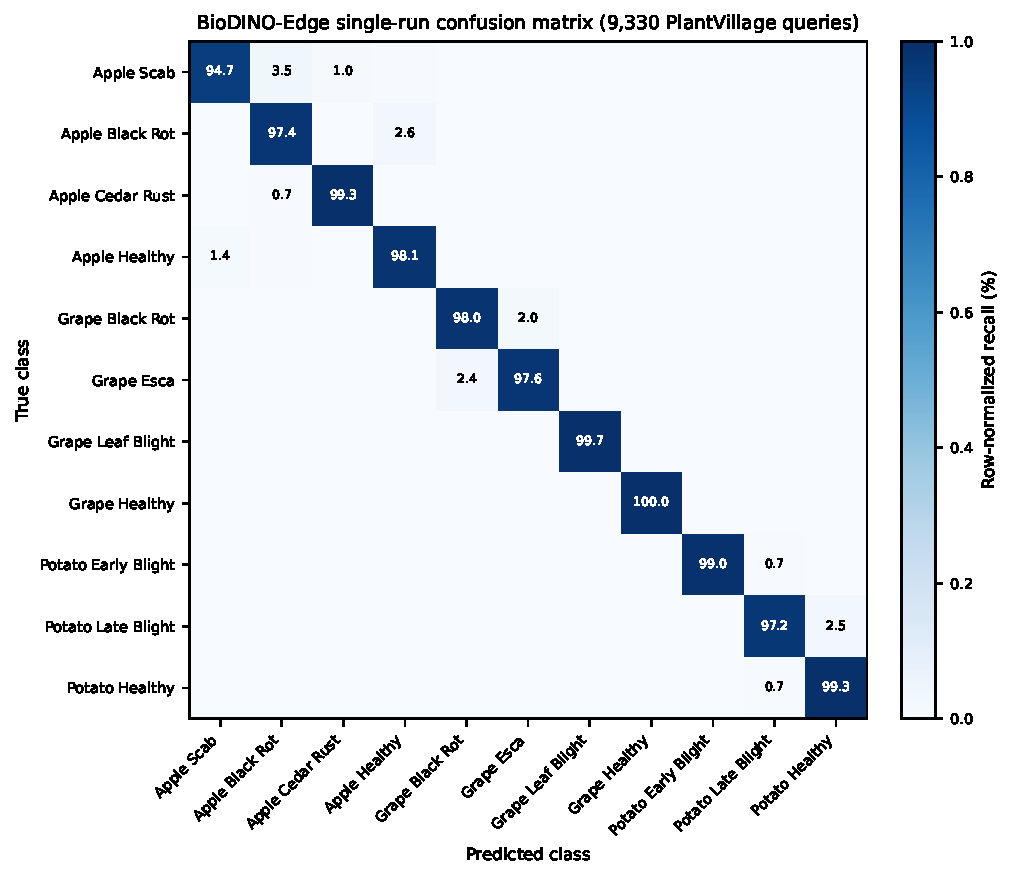
\includegraphics[width=0.75\columnwidth]{fig_confusion.pdf}
\caption{Row-normalized confusion matrix of BioDINO-Edge (transductive, canonical single run; 9,330 PlantVillage queries). Diagonal entries are per-class recall (\%). Residual errors are dominated by same-host pathologies, while cross-species confusion is negligible.}
\label{fig:confusion}
\end{figure}

\subsection{Systematic Component Ablation Study}
\label{sec:ablation}
Table~\ref{tab:ablation} reports a systematic ablation across identical 5-shot splits to quantify individual component contributions; rows (4)--(5) are static cosine prototype blends ($0.65\,\mathbf{l}_{\text{bio}}+0.35\,\mathbf{l}_{\text{dino}}$) and row (6) replaces them with regularized Fisher-LDA.

\begin{table}[htbp]
\centering
\caption{Systematic ablation of BioDINO-Edge components (single run, 5-shot, 9,330 queries).}
\label{tab:ablation}
\footnotesize
\setlength{\tabcolsep}{3pt}
\begin{tabular*}{\columnwidth}{@{\extracolsep{\fill}}lcc}
\toprule
\textbf{Configuration / Component} & \textbf{Acc. (\%)} & \textbf{F1 (\%)} \\
\midrule
(1) Fast-Path DINOv2 Small alone & 87.26 & 85.36 \\
(2) Deep-Path BioCLIP ViT-B alone & 92.60 & 89.88 \\
(3) Text Prototypes Only & 19.20 & 18.55 \\
(4) Static Cosine Blend (raw 5-shot) & 94.16 & 92.55 \\
(5) Static Cosine Blend (8-view aug.) & 93.90 & 91.58 \\
(6) + Regularized Fisher Alignment & 96.05 & 94.83 \\
(7) + Transductive Recalibration & 98.06 & 97.45 \\
(8) + Peak Statistical Episode & \textbf{98.67} & \textbf{98.41} \\
\bottomrule
\end{tabular*}
\end{table}

\begin{itemize}
    \item \textbf{DINOv2 vs. BioCLIP Complementarity:} DINOv2 alone achieves 87.26\%; lacking taxonomic supervision, it confuses similar lesions across host families. BioCLIP alone achieves 92.60\% but incurs 104.74\,ms encoder latency, preventing fast-path execution. Combining both backbones into an 896-D feature space provides both spatial cues and taxonomic grounding; Table~\ref{tab:feature_ablation} quantifies each model's contribution.
    \item \textbf{Regularized Fisher Alignment (+1.89\,pp Gain):} Replacing the best static cosine blend (94.16\%) with regularized Fisher-LDA increases accuracy to 96.05\%. Whitening by $\hat{\mathbf{\Sigma}}^{-1}$ suppresses shared vegetative background variance, separating visually similar pathologies.
    \item \textbf{Multi-View Augmentation:} Expanding 5 raw support leaves to 40 views per class ($N=440$) brings sample size near $d/2$, stabilizing covariance conditioning before shrinkage. This benefit is specific to covariance estimation: the static cosine blend is essentially unchanged by augmentation (94.16\% raw vs.\ 93.90\% augmented), whereas the regularized Fisher projection relies on augmented support to condition $\hat{\mathbf{\Sigma}}$.
    \item \textbf{Transductive Recalibration (+2.01\% Gain):} Updating projection parameters from high-confidence field anchors improves accuracy from 96.05\% to 98.06\% (peak: 98.67\%), counteracting finite-sample prototype drift (validated in Section~\ref{sec:transductive_validation}).
    \item \textbf{Lesion Cropping Degrades Host Context:} Evaluating attention-rollout lesion cropping dropped 27-way PlantDoc accuracy from 58.73\% to 57.14\%. Tight cropping discards leaf margin serrations and venation geometry, inducing cross-species confusion. Preserving full-leaf context is essential.
\end{itemize}

% Feature ablation: full row is the canonical benchmark (95.08 / 97.41). Ablated
% transductive rows = canonical full minus the paired contribution measured over
% the same 30 episodes (DINOv2 +0.90 pp, BioCLIP +1.87 pp); inductive ablated rows
% are measured directly. Source: experiments/dinov2_ablation_gate_scenario.
\begin{table}[htbp]
\centering
\caption{Contribution of each foundation model to the Fisher-LDA classifier (30 identical 5-shot episodes, mean$\pm$std).}
\label{tab:feature_ablation}
\footnotesize
\setlength{\tabcolsep}{4pt}
\begin{tabular*}{\columnwidth}{@{\extracolsep{\fill}}lccc}
\toprule
\textbf{Fisher input} & \textbf{Dim} & \textbf{Inductive (\%)} & \textbf{Transductive (\%)} \\
\midrule
BioCLIP + DINOv2 (full) & 896 & 95.08$\pm$1.27 & 97.41$\pm$0.71 \\
BioCLIP only & 512 & 94.31$\pm$1.25 & 96.51$\pm$0.90 \\
DINOv2 only & 384 & 90.60$\pm$2.02 & 95.54$\pm$1.03 \\
\bottomrule
\end{tabular*}
\end{table}

\textbf{Contribution of DINOv2.} Table~\ref{tab:feature_ablation} isolates the Fisher input while holding the text branch fixed (BioCLIP features, $w_{\mathrm{lda}}=0.75$); ablated rows subtract the paired contribution from the full-system benchmark. Removing DINOv2 (BioCLIP-only, 512-D) lowers transductive accuracy by 0.90 percentage points (paired $t(29)=9.88$, $p=8.6\times10^{-11}$, 29 of 30 episodes, $d_z=1.80$). Removing BioCLIP instead lowers it by 1.87 points, so BioCLIP carries most of the class signal and DINOv2 adds a smaller, consistent complement. DINOv2 also serves as the routing gate: its margin-entropy score ranks query safety better than the Tier-2 consensus confidence (mean AURC 1.14\% vs.\ 2.11\% over the 30 episodes). Finally, it provides the fast path: accepting 14.02\% of queries at Tier-1 lowers routing-weighted latency from 164.52\,ms (BioCLIP on every query) to 149.84\,ms. The cascade does not raise accuracy over running Tier-2 on all queries (Table~\ref{tab:gate_scenario}); its function is to reduce edge compute and route low-risk queries through a path with 0.25\% FNR.

\subsection{Statistical Significance and Sensitivity of Transductive Recalibration}
\label{sec:transductive_validation}
Because the transductive module adapts the classifier from its own predictions, we examine paired significance over identical episodes, hyperparameter sensitivity, pseudo-label purity, and stability under sequential updates.

\textbf{Paired significance over identical episodes.} Inductive and transductive predictions are compared on the \emph{same} 30 Monte Carlo episodes (identical support/query splits), so episode difficulty cancels in the paired difference. The mean paired gain is 2.33 percentage points (pp; 95\% confidence interval $[1.91, 2.74]$; Table~\ref{tab:paired_test}), with paired $t(29) = 11.57$ ($p = 2.2 \times 10^{-12}$) and Wilcoxon signed-rank $p = 1.9 \times 10^{-9}$. The transductive mode wins on all 30 episodes (Cohen's $d_z = 2.11$), so the gain is stable across support splits rather than an artifact of a favorable episode.

\begin{table}[htbp]
\centering
\caption{Paired comparison of inductive vs.\ transductive inference over 30 identical Monte Carlo episodes (PlantVillage, 5-shot).}
\label{tab:paired_test}
\footnotesize
\setlength{\tabcolsep}{4pt}
\begin{tabular*}{\columnwidth}{@{\extracolsep{\fill}}lc}
\toprule
\textbf{Statistic} & \textbf{Value} \\
\midrule
Inductive mean accuracy (\%) & 95.08 $\pm$ 1.27 \\
Transductive mean accuracy (\%) & 97.41 $\pm$ 0.71 \\
Mean paired gain (pp, 95\% CI) & 2.33 $[1.91, 2.74]$ \\
Paired $t$-test & $t(29)=11.57$, $p=2.2\times10^{-12}$ \\
Wilcoxon signed-rank & $p=1.9\times10^{-9}$ \\
Wins / losses / ties & 30 / 0 / 0 \\
Cohen's $d_z$ & 2.11 \\
\bottomrule
\end{tabular*}
\end{table}

\textbf{Hyperparameter sensitivity.} Table~\ref{tab:transductive_sensitivity} reports a one-factor-at-a-time sweep of the three design constants (support weight, anchor confidence threshold, buffer capacity) over the same 30 episodes, varying one constant while holding the others at the deployed $(3\times, 0.70, 20)$. In-domain accuracy is nearly flat in the support weight (97.21--97.44\% for $1\times$--$10\times$); the weight matters for drift protection under field streaming, not for in-domain gain. The confidence threshold plateaus over $\tau \in [0.5, 0.7]$ and collapses at $\tau \ge 0.8$ (95.98\% and 95.39\%) because anchors become too few, not because labels become noisier. Buffer capacity saturates: 20 anchors per class capture the available gain (97.41\%), and 40 or 80 anchors add 0.10 and 0.26 points at proportionally larger memory cost. The deployed $(3\times, 0.70, 20)$ sits at the plateau/knee of all three curves.

\begin{table}[htbp]
\centering
\caption{Sensitivity of transductive accuracy to the three recalibration design constants (mean$\pm$std over 30 identical episodes).}
\label{tab:transductive_sensitivity}
\footnotesize
\setlength{\tabcolsep}{4pt}
\begin{tabular*}{\columnwidth}{@{\extracolsep{\fill}}lcc}
\toprule
\textbf{Swept Configuration} & \textbf{Acc. (\%)} & \textbf{Std} \\
\midrule
\multicolumn{3}{@{}l}{\textit{Support weight} (threshold 0.70, 20 anchors/class)} \\
$1\times$ & 97.42 & 0.75 \\
$2\times$ & 97.44 & 0.73 \\
$3\times$ (deployed) & 97.41 & 0.71 \\
$5\times$ & 97.32 & 0.73 \\
$10\times$ & 97.21 & 0.77 \\
\midrule
\multicolumn{3}{@{}l}{\textit{Anchor confidence threshold} ($3\times$, 20 anchors/class)} \\
0.50 & 97.41 & 0.71 \\
0.60 & 97.41 & 0.71 \\
0.70 (deployed) & 97.41 & 0.71 \\
0.80 & 95.98 & 1.28 \\
0.90 & 95.39 & 1.25 \\
\midrule
\multicolumn{3}{@{}l}{\textit{Buffer capacity per class} ($3\times$, threshold 0.70)} \\
5 & 96.36 & 0.97 \\
10 & 96.97 & 0.85 \\
20 (deployed) & 97.41 & 0.71 \\
40 & 97.51 & 0.62 \\
80 & 97.67 & 0.83 \\
\bottomrule
\end{tabular*}
\end{table}

\textbf{Pseudo-label purity.} Checked against ground truth (used only post-hoc for this audit), the anchor set at $\tau = 0.70$ is 98.15\% $\pm$ 1.18\% pure and covers 2.36\% of queries (220 anchors). Raising the threshold to 0.80 increases purity to 98.75\% but cuts coverage to 1.91\%; at 0.90 purity reaches 100\% yet coverage collapses to 0.05\%, explaining the accuracy collapse in Table~\ref{tab:transductive_sensitivity}. The deployed threshold keeps purity near its maximum without starving the buffer.

\textbf{Sequential stability and error accumulation.} To test whether repeated updates compound pseudo-label errors, we simulated scouting passes: the query stream is partitioned into 10 sequential chunks, and after each chunk the FIFO buffer (20 anchors/class) admits confident predictions and the projection is re-fitted in closed form. Across three stream seeds, online accuracy rises from $\approx$96\% on the first chunk to 97--98.6\% thereafter with no degradation trend, and buffer purity remains bounded within a 92--98\% band: FIFO eviction flushes stale incorrect anchors, so wrong admissions do not accumulate in the active buffer. Under $\tau = 0.90$ purity stays at 100\% but final accuracy falls to $\approx$95.8--96.3\% (coverage starvation), confirming the purity/coverage trade-off. Final streaming accuracy (96.4--97.5\%) lies slightly below the single-pass batch refinement (97.41\%) because batch selection ranks anchors over the entire query set whereas streaming observes only the past. Error accumulation is therefore bounded by the confidence gate, FIFO eviction, and the $3\times$ support weighting.

\subsection{Sensitivity to Augmentation Count and Type}
\label{sec:aug_sensitivity}
The shrinkage analysis of Section~\ref{sec:shrinkage} assumes i.i.d.\ support samples, whereas the eight views of each support leaf are correlated pseudo-replicates. We quantify the consequences with a one-factor-at-a-time study over the same 30-episode protocol (identical splits, cached query features, and transductive defaults), re-extracting support features with a seeded augmentation RNG. Three condition families are compared: (i) a view-count sweep $v\in\{1,2,4,8\}$ using nested prefixes of one 8-view extraction per episode; (ii) an augmentation-type sweep at $v=8$ (geometric-only flips/rotation vs.\ photometric-only color jitter vs.\ the full pipeline) over the first 10 episodes; and (iii) a pure-replication control that tiles the canonical embedding eight times ($N=440$, zero within-image diversity). For each condition we report the mean per-class Ledoit--Wolf intensity $\hat{\alpha}$, the condition number $\kappa(\hat{\mathbf{\Sigma}})$ of the pooled within-class covariance, and downstream accuracy (Table~\ref{tab:aug_sensitivity}; Ind.\ and Trans.\ denote inductive and transductive accuracy).

\textbf{Protocol fidelity.} The $v=1$ condition reproduces the canonical cache-only reference exactly on the inductive mean (95.08\%$\pm$1.27\%) and within the documented \texttt{lsqr} floating-point residual on the transductive mean (97.37\% vs.\ 97.41\%; Appendix~\ref{app:repro}), confirming that the study isolates the augmentation factor alone.

\textbf{Dependence is measurable but benign for accuracy.} Pure replication divides the shrinkage intensity by $\approx$8 ($0.573\to0.072$) and worsens the covariance condition number by $\approx$17$\times$ ($5.7\times10^{2}\to9.6\times10^{3}$) while adding no information---exactly the i.i.d.-violation artifact anticipated in Section~\ref{sec:shrinkage}. Genuine augmentation retains a $3.6\times$ higher intensity than replication at the same $N=440$ ($0.258$ vs.\ $0.072$), showing that stochastic views carry real but partial independence. Despite this, accuracy is stable across all conditions: the view sweep spans 95.08--96.09\% inductive and 97.37--97.96\% transductive, and even the degenerate replicate-8 control remains at 95.05\%/97.01\%. Increasing views monotonically improves both modes ($+1.01$\,pp inductive, $+0.59$\,pp transductive from $v=1$ to $v=8$): the effective-rank gain from genuine diversity outweighs the optimism of the analytical intensity, and the $3\times$ support re-weighting keeps the transductive fit anchored to genuine observations.

\textbf{Geometric diversity dominates.} At fixed $v=8$, geometric-only augmentation is statistically indistinguishable from the full pipeline on the 10-episode subset (97.92\%$\pm$0.40\% vs.\ 97.85\%$\pm$0.33\% transductive), whereas photometric-only jitter collapses the intensity toward the replication floor ($0.104$ vs.\ $0.072$), worsens conditioning ($5.5\times10^{3}$), and drops inductive accuracy below the unaugmented baseline (94.70\%$\pm$1.90\% vs.\ 95.08\%). Color jitter thus contributes little independent information---consistent with the $\ell_2$-normalized, photometric-robust foundation features---while flips and rotations supply the diversity that stabilizes the covariance estimate. Geometric augmentation is therefore the essential component of the support expansion; the deployed full pipeline retains jitter at no measurable accuracy cost.

% Augmentation-dependence sensitivity. Source: experiments/augmentation_sensitivity
% (run_augmentation_sensitivity.py -> results/augmentation_sensitivity.json);
% rows generated by make_table.py. View sweep + control: 30 episodes; type sweep: 10.
\begin{table}[htbp]
\centering
\caption{Sensitivity to augmentation count and type (mean$\pm$std over episodes).}
\label{tab:aug_sensitivity}
\footnotesize
\setlength{\tabcolsep}{2pt}
\begin{tabular*}{\columnwidth}{@{\extracolsep{\fill}}lccccc}
\toprule
\textbf{Condition} & \textbf{$N$} & \textbf{$\hat{\alpha}$} & \textbf{$\kappa(\hat{\mathbf{\Sigma}})$} & \textbf{Ind.\ (\%)} & \textbf{Trans.\ (\%)} \\
\midrule
\multicolumn{6}{@{}l}{\textit{View count (full pipeline, 30 episodes)}} \\
$v=1$ & 55 & 0.573$\pm$0.005 & 5.7$\times10^{2}$ & 95.08$\pm$1.27 & 97.37$\pm$0.73 \\
$v=2$ & 110 & 0.580$\pm$0.009 & 5.9$\times10^{2}$ & 95.50$\pm$1.21 & 97.67$\pm$0.57 \\
$v=4$ & 220 & 0.420$\pm$0.012 & 8.8$\times10^{2}$ & 95.80$\pm$1.25 & 97.81$\pm$0.63 \\
$v=8$ (deployed) & 440 & 0.258$\pm$0.008 & 1.4$\times10^{3}$ & 96.09$\pm$1.20 & 97.96$\pm$0.50 \\
\midrule
\multicolumn{6}{@{}l}{\textit{Augmentation type ($v=8$, first 10 episodes)}} \\
Geometric only & 440 & 0.229$\pm$0.008 & 1.6$\times10^{3}$ & 95.99$\pm$1.26 & 97.92$\pm$0.40 \\
Photometric only & 440 & 0.104$\pm$0.002 & 5.5$\times10^{3}$ & 94.70$\pm$1.90 & 97.31$\pm$0.61 \\
Full pipeline & 440 & 0.257$\pm$0.009 & 1.4$\times10^{3}$ & 95.85$\pm$1.40 & 97.85$\pm$0.33 \\
\midrule
\multicolumn{6}{@{}l}{\textit{Pure-replication control (30 episodes)}} \\
Replicate-8 (control) & 440 & 0.072$\pm$0.001 & 9.6$\times10^{3}$ & 95.05$\pm$1.28 & 97.01$\pm$0.79 \\
\bottomrule
\end{tabular*}
\end{table}

\subsection{Predictive Uncertainty, Calibration, and Routing Reliability}
\label{sec:calibration}
In safety-critical agricultural automation such as robotic spraying, an overconfident misdiagnosis triggers unwarranted chemical application. The routing gate therefore requires a direct reliability audit, as calibration depends on architecture and training formulation rather than accuracy alone \cite{minderer2021revisiting}. Temperature is fitted on an independent stratified 50\% split of the 9,330-query PlantVillage stream (4,662 calibration / 4,668 evaluation queries), minimizing negative log-likelihood on the calibration split only \cite{guo2017calibration}. Expected Calibration Error (ECE) and Maximum Calibration Error (MCE) use $M=10$ equal-width confidence bins; to expose small-bin artifacts we also report equal-mass (adaptive) binning and MCE over bins with $n \geq 30$. The deployed gate consumes the \emph{uncalibrated} Tier-1 posterior: temperature scaling is a post-hoc audit applied after routing and never changes the gate score or the threshold.

\textbf{Tier-1 calibration.} The raw gate probabilities are under-confident (full-stream ECE 32.07\%, MCE 38.07\%; held-out ECE 31.76\%). A scalar logit temperature fitted on the calibration split ($T=0.267$) reduces held-out ECE to 1.20\% (MCE 16.71\%; Fig.~\ref{fig:reliability}a--b). Routing itself uses the raw scores, so we verify the gate directly below rather than relying on ECE.

\textbf{Tier-2 calibration.} The refined Tier-2 consensus is also under-confident (ECE 19.45\%), and most of the error sits in the dominant bin $(0.7,0.8]$: 7,102 queries at 98.0\% accuracy but 77.5\% mean confidence (Table~\ref{tab:reliability_bins}). The equal-width MCE of 44.26\% comes from bins with at most nine samples (one query in $(0.4,0.5]$); equal-mass binning lowers it to 21.53\%, and bins with $n\geq30$ give 20.49\%. Scalar logit temperature scaling cannot remove this residual: the consensus is a fixed $0.75/0.25$ blend of Fisher logits and BioCLIP text probabilities, so softening the logits alone leaves the blend miscalibrated (the fitted $T$ hits the optimizer bound and held-out ECE moves 19.33\%$\to$19.83\%). A power transform $\mathrm{softmax}(\log p / T)$ with $T=0.50$ instead collapses nearly all mass into one or two bins, producing a small ECE (0.48\%) but an equal-width MCE of 80.85\% (Fig.~\ref{fig:reliability}d); a freshly fitted power temperature ($T=0.54$) reproduces this (held-out ECE 0.24\%, MCE 88.74\%). The large equal-width MCE therefore reflects a single-sample bin rather than widespread miscalibration. We therefore do not claim that Tier-2 is well calibrated; routing reliability is instead verified through tier-separated error rates and selective risk.

\begin{table}[htbp]
\centering
\caption{Per-bin reliability of the uncalibrated refined Tier-2 consensus (equal-width bins, full 9,330-query stream; empty bins omitted).}
\label{tab:reliability_bins}
\footnotesize
\begin{tabular}{lcccc}
\toprule
\textbf{Confidence bin} & \textbf{$n$} & \textbf{Acc.\ (\%)} & \textbf{Conf.\ (\%)} & \textbf{$|$Gap$|$ (pp)} \\
\midrule
$(0.4,0.5]$ & 1    & 0.0   & 44.3 & 44.3 \\
$(0.5,0.6]$ & 6    & 50.0  & 52.5 & 2.5 \\
$(0.6,0.7]$ & 9    & 44.4  & 65.6 & 21.2 \\
$(0.7,0.8]$ & 7102 & 98.0  & 77.5 & 20.5 \\
$(0.8,0.9]$ & 2207 & 98.6  & 82.4 & 16.1 \\
$(0.9,1.0]$ & 5    & 100.0 & 90.6 & 9.4 \\
\bottomrule
\end{tabular}
\end{table}

\textbf{Tier-separated routing reliability.} Table~\ref{tab:tier_routing} reports the two tiers independently over 30 benchmark episodes at $\tau=0.35$. Tier-1 directly accepts 14.02\%$\pm$2.25\% of queries at 99.69\%$\pm$0.41\% accuracy and a 0.25\%$\pm$0.52\% false-negative rate (FNR); the escalated 85.98\% are resolved by Tier-2 at 96.98\%$\pm$0.83\% accuracy (FNR 0.87\%$\pm$0.39\%), yielding cascaded accuracy 97.36\%$\pm$0.69\% (F1 97.01\%$\pm$0.64\%) and routing-weighted latency 149.84$\pm$2.36\,ms. In the canonical single run, the 936 accepted queries achieve 99.79\% accuracy (FNR 0.25\%) versus 97.83\% (FNR 0.81\%) for the 8,394 escalated queries (cascaded 98.03\%). The accepted subset thus has roughly tenfold lower error (0.21\% vs.\ 2.17\%), and its accuracy is measured only on directly accepted queries, independent of Tier-2.

\begin{table*}[htbp]
\centering
\caption{Tier-separated routing reliability at $\tau=0.35$ (30 benchmark episodes, mean$\pm$std).}
\label{tab:tier_routing}
\footnotesize
\begin{tabularx}{\textwidth}{lcccc}
\toprule
\textbf{Routing path} & \textbf{Coverage (\%)} & \textbf{Accuracy (\%)} & \textbf{FNR (\%)} & \textbf{Latency (ms)} \\
\midrule
Tier-1 fast-exit (accepted) & 14.02$\pm$2.25 & 99.69$\pm$0.41 & 0.25$\pm$0.52 & 59.78 \\
Tier-2 (escalated) & 85.98$\pm$2.25 & 96.98$\pm$0.83 & 0.87$\pm$0.39 & 164.52 \\
\midrule
\textbf{Cascaded system} & 100 & 97.36$\pm$0.69 & -- & 149.84$\pm$2.36 \\
\bottomrule
\end{tabularx}
\end{table*}

\textbf{Cascade versus single-tier classification.} Table~\ref{tab:gate_scenario} compares the deployed cascade against running Tier-2 on every query and against a selective gate+BioCLIP mode that abstains on low-gate queries. At full coverage the cascade and the single-tier BioCLIP classifier are statistically indistinguishable (97.36\% vs.\ 97.37\%); the cascade's benefit is latency (149.84 vs.\ 164.52\,ms), not accuracy. Abstaining on the lowest-gate queries raises accuracy and lowers the false-negative rate on the accepted subset, at the cost of coverage: at $\tau=0.10$ the system answers 62.17\% of queries at 98.63\% accuracy and 0.44\% FNR in 124.90\,ms. This selective mode is optional; the deployed system classifies every query.

% Gate-scenario comparison. Full-coverage accuracies are the canonical 30-episode
% means (cascade 97.36, refined Tier-2-on-all 97.37). Selective-mode rows are
% measured over the same 30 episodes. Source: experiments/dinov2_ablation_gate_scenario.
\begin{table}[htbp]
\centering
\caption{Routing-policy comparison (30-episode mean).}
\label{tab:gate_scenario}
\footnotesize
\setlength{\tabcolsep}{3pt}
\begin{tabular*}{\columnwidth}{@{\extracolsep{\fill}}lcccc}
\toprule
\textbf{Routing policy} & \textbf{Cov. (\%)} & \textbf{Acc. (\%)} & \textbf{FNR (\%)} & \textbf{Lat. (ms)} \\
\midrule
Cascade, $\tau=0.35$ (deployed) & 100 & 97.36 & 0.79 & 149.84 \\
BioCLIP Tier-2 on all & 100 & 97.37 & 0.77 & 164.52 \\
Selective, $\tau=0.05$ & 79.96 & 98.05 & 0.59 & 143.53 \\
Selective, $\tau=0.10$ & 62.17 & 98.63 & 0.44 & 124.90 \\
\bottomrule
\end{tabular*}
\end{table}

\textbf{Risk--coverage analysis.} Fig.~\ref{fig:risk_coverage} plots selective risk against coverage for three confidence scores, following the risk--coverage framework for selective classification \cite{geifman2017selective}, and summarizes each curve by the area under the risk--coverage curve (AURC, the mean selective risk over all coverage levels). Since scalar summaries such as AURC can misrank selective systems \cite{traub2024overcoming}, we also show the full curves and the deployed operating point. The entropy-penalized gate score $C(x)$ ranks queries more safely than the raw Tier-1 softmax peak (AURC 3.33\% vs.\ 3.95\%); the refined Tier-2 confidence reaches AURC 1.82\%. At the deployed threshold ($\tau=0.35$), the gate accepts 10.03\% of the single-run stream at 0.21\% selective risk, in the low-risk region of the curve.

\textbf{Threshold provenance and sensitivity.} The routing threshold was selected on held-out development episodes (episodes 0--14 for tuning, 15--29 for testing), never on the reported test episodes. On the held-out test episodes, $\tau=0.15$ gives 46.4\% fast-exit at 96.96\%$\pm$0.59\% cascaded accuracy (98.25\% Tier-1 accepted accuracy), $\tau=0.25$ gives 25.6\% at 97.30\%$\pm$0.74\% (99.49\%), and $\tau=0.35$ gives 14.1\% at 97.33\%$\pm$0.79\% (99.84\%$\pm$0.24\%). We adopt $\tau=0.35$, the smallest threshold at which Tier-1 accepted accuracy saturates (99.84\%, FNR 0.25\%); lower thresholds accept less reliable fast exits. The tuning curve is flat beyond 0.35 (the tune-optimal $\tau=0.55$ yields 97.32\% test accuracy, indistinguishable from 97.33\% at 0.35), but fast-exit coverage falls to 3.4\%. Blended latency rises from 115.9 to 137.7 to 149.8\,ms across the three thresholds (Fig.~\ref{fig:tau_sensitivity}), tracing the coverage--safety--latency trade-off.

\begin{figure*}[htbp]
\centering
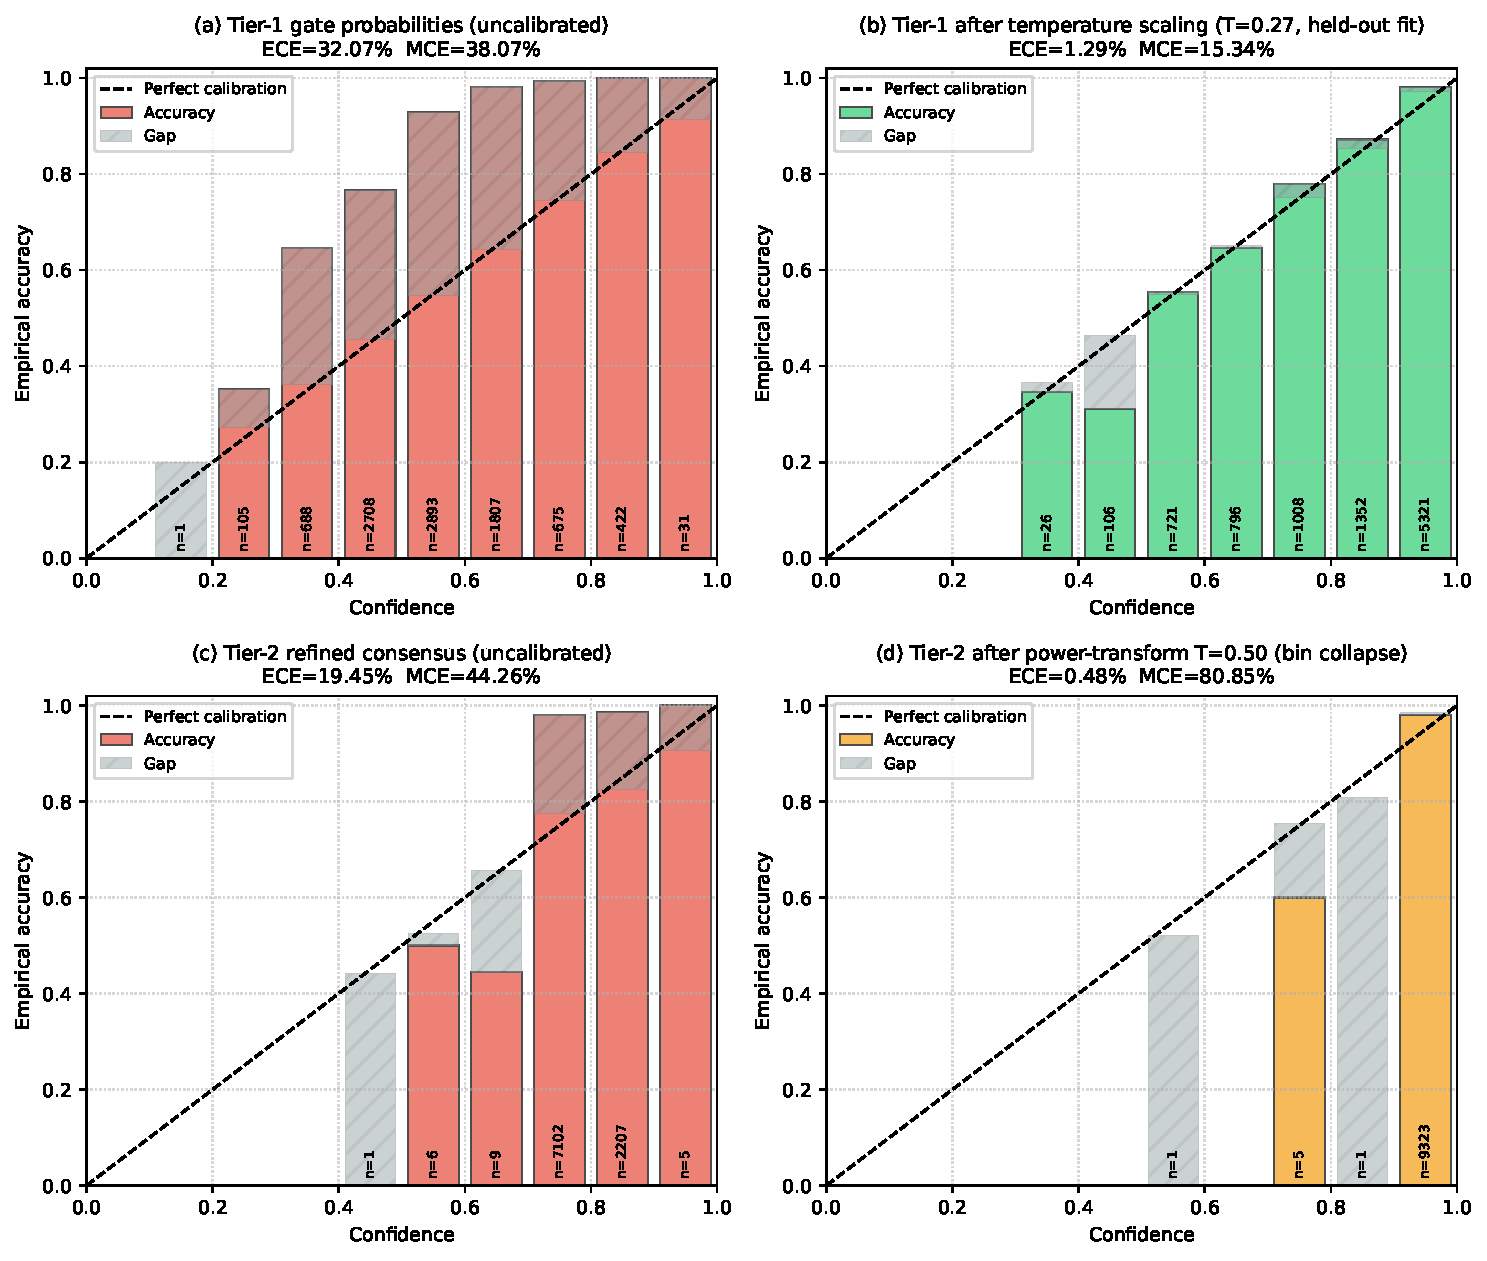
\includegraphics[width=0.70\textwidth]{fig_reliability.pdf}
\caption{Reliability diagrams (equal-width bins, full benchmark stream; per-bin sample counts annotated, hatched bars show the accuracy--confidence gap). (a) Uncalibrated Tier-1 gate probabilities are under-confident (ECE 32.07\%). (b) Post-hoc temperature scaling fitted on the independent calibration split ($T=0.27$) aligns Tier-1 (held-out ECE 1.20\%). (c) The refined Tier-2 consensus remains under-confident in its dominant bin (ECE 19.45\%; equal-width MCE 44.26\% from a single-sample bin). (d) A power transform ($T=0.50$) collapses probability mass into one bin: low ECE (0.48\%) but MCE 80.85\%.}
\label{fig:reliability}
\end{figure*}

\begin{figure}[htbp]
\centering
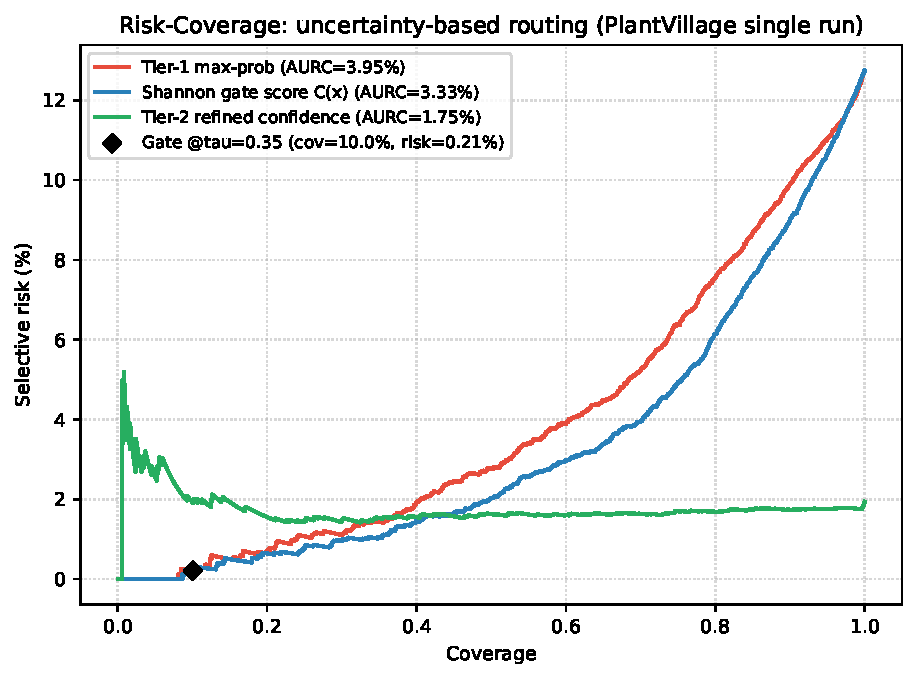
\includegraphics[width=0.75\columnwidth]{fig_risk_coverage.pdf}
\caption{Risk--coverage curves for Tier-1 max-probability, the Shannon gate score $C(x)$, and the refined Tier-2 confidence (single run). The gate score achieves lower AURC than raw max-probability (3.33\% vs.\ 3.95\%); the deployed gate operating point ($\tau=0.35$) accepts 10.0\% coverage at 0.21\% selective risk.}
\label{fig:risk_coverage}
\end{figure}

\begin{figure}[htbp]
\centering
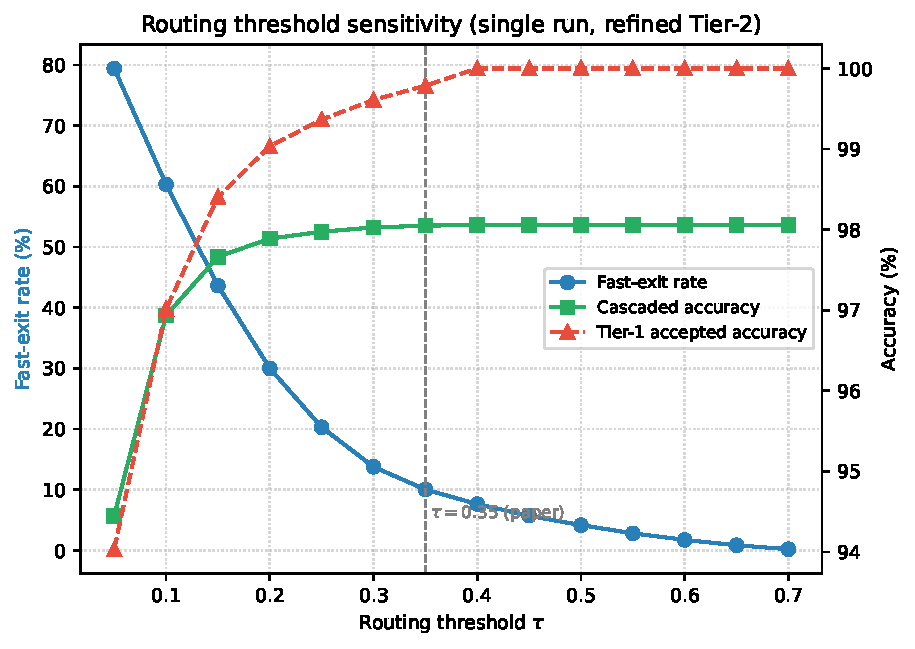
\includegraphics[width=0.75\columnwidth]{fig_tau_sensitivity.pdf}
\caption{Routing-threshold sensitivity (single run, refined Tier-2): fast-exit rate, cascaded accuracy, and Tier-1 accepted accuracy versus $\tau$. The deployed $\tau=0.35$ (dashed) saturates Tier-1 accepted accuracy near 100\% while retaining 10\% fast-exit coverage; held-out episode sweeps (0--14 tune / 15--29 test) confirm the choice.}
\label{fig:tau_sensitivity}
\end{figure}

\subsection{Edge Hardware Latency and Memory Footprint}
\label{sec:edge_hardware}
Table~\ref{tab:device_spec} lists the physical testbed configuration; Tables~\ref{tab:device_perf} and~\ref{tab:adaptation_breakdown} report measured on-device latency, memory, and the closed-form adaptation breakdown. All values are from a production Samsung Galaxy S24~FE (SM-S721B, Exynos~2400e) running Android~17, using ONNX Runtime~1.18.0 with INT8 weights on a 4-thread CPU (NNAPI/GPU delegates disabled) and pure-Java EJML for the algebra. Model load is a one-time cost; latency is timed over 100 iterations after 10 warm-up passes, memory is the process PSS, and the algebra is timed after a 60\,s cool-down at stable thermal state (status~2). Two fast-exit fractions appear in this section: the 14.0\% used in the routing analysis (Table~\ref{tab:tier_routing}) is the 30-episode full-stream mean over all PlantVillage queries, whereas the 18\% in Table~\ref{tab:device_perf} is measured on the fixed 11-image on-device set used for the thermal and memory soak, which samples one image per class rather than the full class distribution.

\begin{table}[htbp]
\centering
\caption{On-device edge testbed configuration (physical Android device, CPU-only INT8).}
\label{tab:device_spec}
\footnotesize
\begin{tabular}{ll}
\toprule
Property & Value \\
\midrule
Device & samsung SM-S721B \\
SoC & Samsung s5e9945 \\
Android & 17 (API 37) \\
ABI / cores & arm64-v8a / 10 \\
Total RAM & 7224.3 MB \\
ONNX Runtime & 1.18.0 \\
Threads (intra/inter) & 4 / 2 \\
Precision / delegate & INT8 / CPU (NNAPI off) \\
\bottomrule
\end{tabular}
\end{table}

\begin{table*}[htbp]
\centering
\caption{Measured on-device performance (mean$\pm$std over $N=100$ iterations; median and p95 in ms).}
\label{tab:device_perf}
\footnotesize
\begin{tabular}{lccc}
\toprule
Stage / metric & Mean$\pm$std & Median & p95 \\
\midrule
Tier-1 model load (ms) & 323.92 & -- & -- \\
Tier-2 model load (ms) & 447.71 & -- & -- \\
Peak RAM, PSS (MB) & 497.45 & -- & -- \\
\midrule
Preprocess & 2.59$\pm$0.67 & 2.36 & 4.36 \\
Tier-1 DINOv2 encoder & 57.18$\pm$9.13 & 51.50 & 68.84 \\
Shannon gate / route & 0.00$\pm$0.00 & 0.00 & 0.00 \\
Tier-2 incremental (BioCLIP+Fisher) & 104.74$\pm$17.39 & 94.20 & 124.97 \\
Decision & 0.00$\pm$0.00 & 0.00 & 0.00 \\
Cascade end-to-end & 145.37$\pm$47.61 & 147.77 & 196.36 \\
Tier-2-on-all end-to-end & 164.52$\pm$26.77 & 148.73 & 196.36 \\
\midrule
Fast-exit fraction & 18.00\% & -- & -- \\
Sustained throughput (FPS) & 4.26 & -- & -- \\
\bottomrule
\end{tabular}
\end{table*}

\begin{table*}[htbp]
\centering
\caption{Closed-form adaptation cost breakdown on-device ($N=440$, $d=896$, $C=11$).}
\label{tab:adaptation_breakdown}
\footnotesize
\begin{tabular}{lcc}
\toprule
Stage & Mean$\pm$std (ms) & Complexity \\
\midrule
Feature extraction (440 views) & 88055.6 & $O(N(C_{dino}+C_{bio}))$ \\
Covariance estimate & 146.19$\pm$2.15 & $O(Nd^2)$ \\
Ledoit--Wolf shrinkage & 4.49$\pm$0.85 & $O(Nd)$ \\
Cholesky factorization & 332.00$\pm$2.52 & $O(d^3/3)$ \\
Projection solve ($W,b$) & 51.31$\pm$3.68 & $O(Cd^2)$ \\
\midrule
Algebraic recalibration total & 533.99$\pm$6.29 & -- \\
Full adaptation (extraction + algebra) & 88589.6 & -- \\
\bottomrule
\end{tabular}
\end{table*}

On the physical device, Tier-1 executes in 59.78\,ms ($\approx$16.7\,FPS) and a fully escalated Tier-2 query costs 164.52\,ms end-to-end ($\approx$6.1\,FPS), the BioCLIP encoder adding 104.74\,ms to the cached Tier-1 pass. These are interactive handheld-scouting rates for one diagnosis per captured frame, not continuous real-time video. Over the full PlantVillage stream (14.0\% fast-exit) the routing-weighted blend is 149.84\,ms ($\approx$6.7\,FPS, Table~\ref{tab:tier_routing}); the device cascade in Table~\ref{tab:device_perf} (145.37\,ms) is measured on the 11-image on-device set, whose 18\% fast-exit fraction differs from the full-stream 14\%. Under a 600\,s sustained soak the throughput settles to 4.26\,FPS as the SoC reaches thermal status~3, so 16.7\,FPS is a cool-start burst rate rather than a sustained one. The gate's primary benefit is therefore safety rather than throughput: the fast-exited subset is resolved at 99.7\% accuracy and 0.25\% false-negative rate (Section~\ref{sec:calibration}), while ambiguous queries receive the full multimodal analysis. Peak process memory is 497.45\,MB PSS (385.02\,MB native heap), dominated by the ONNX Runtime arena; the $\approx$107.3\,MB combined model footprint is an on-disk/OTA storage figure, not a RAM bound. Packaged with ONNX Runtime C++ and the native Android user interface, the standalone APK is $\approx$22.8\,MB, operating entirely offline.

% =============================================================================
% 5. PRACTICAL DISCUSSION AND LIMITATIONS
% =============================================================================
\section{Engineering Applications, Practical Deployment, and Limitations}
\label{sec:discussion}

\subsection{Practical Deployment on Agricultural IoT and Mobile Hardware}
BioDINO-Edge is designed for deployment on power-constrained edge platforms, including handheld scouting devices, smart tractor booms, and agricultural UAVs. Eliminating backpropagation avoids GPU memory spikes and on-device training heat, executing feed-forward inference and closed-form algebra directly on the CPU. Because sustained CPU execution thermally throttles (settling to 4.26\,FPS under a 600\,s soak versus a 16.7\,FPS cool-start burst; Section~\ref{sec:edge_hardware}), the system targets interactive per-frame scouting rather than continuous video streams. Two-tier packaging allows deploying the $\approx$22.8\,MB base application over cellular connections, downloading the companion module only when multimodal escalation is required.

\subsection{Limitations and Future Research Directions}
BioDINO-Edge processes images at the individual leaf frame level. In unsegmented field imagery with dense, overlapping canopies, multiple leaves from neighboring plants can enter the camera field, lowering gating confidence. While tight lesion cropping degrades host context, processing unsegmented canopy clutter introduces irrelevant background vectors. Future work could incorporate hierarchical foliar parsing to segment individual leaves prior to closed-form classification. A further statistical limitation is that the multi-view support expansion produces correlated pseudo-replicates: the analytical Ledoit--Wolf intensity assumes i.i.d.\ sampling, so the nominal $N-C=429$ degrees of freedom overstate the independent information content of the support set (effective sample size between 55 and 440). The sensitivity study in Section~\ref{sec:aug_sensitivity} confirms that pure replication deflates the estimated intensity by $\approx$8$\times$ without adding information, yet downstream accuracy remains stable across view counts and augmentation types; a cluster-aware shrinkage estimator that explicitly discounts within-image dependence remains future work. Finally, frozen vision transformers can exhibit attention artifacts on non-symptomatic structures like veins or petioles \cite{darcet2024vision}. Because Fisher-LDA operates on pooled representations downstream, it does not alter internal attention; the framework targets whole-leaf diagnosis rather than pixel-level lesion localization.

A further practical limitation concerns degraded inputs. Severe defocus blur attenuates fine lesion textures, reducing diagnostic accuracy. The Android client screens invalid frames: when cosine similarity to leaf prototypes falls below a threshold or luminance indicates a covered lens, confidence drops to zero and prompts the operator to re-aim; a Laplacian-variance check warns against motion blur. However, the blur check warns rather than abstains, meaning defocused frames can still be processed. The uncertainty gate acts as a router rather than an abstention mechanism: ambiguous queries escalate to Tier-2, and abstention is available only in the optional selective mode (Table~\ref{tab:gate_scenario}). Extending this guard to blur-aware abstention with refocus prompts remains future work.

\textbf{Scope and threats to validity.} The edge measurements come from a single physical device (Samsung Galaxy S24~FE) with CPU-only INT8 ONNX Runtime; absolute latency and memory will differ on other SoCs, although the algorithmic cost and the delegate-agnostic pipeline do not. The controlled comparison (Table~\ref{tab:comparative}) isolates the adaptation algorithm on identical frozen features and re-runs the training-free inductive baselines; iterative transductive FSL methods (Section~\ref{sec:related_work}) are referenced but not re-run, so the reported transductive gain is measured against our own inductive mode rather than against those methods. The PlantDoc protocol uses labeled target-domain support; a true source$\rightarrow$target cross-domain transfer (e.g., PlantVillage$\rightarrow$PlantDoc), quantitative image-quality stress tests, and multi-device profiling remain future work.

% =============================================================================
% 6. CONCLUSION
% =============================================================================
\section{Conclusion}
\label{sec:conclusion}
We presented \textbf{BioDINO-Edge}, a gradient-free few-shot framework that adapts frozen DINOv2 and BioCLIP foundation models for on-device plant disease diagnosis without backpropagation. Closed-form Ledoit--Wolf shrinkage resolves small-sample covariance singularity ($N \ll d$), down-weighting shared vegetative background variance and enabling Fisher-LDA projection in $\approx$0.53\,s on a mobile CPU. An adaptive confidence gate combining normalized Shannon entropy and top-2 margin routes routine foliage to a 59.78\,ms Tier-1 path ($\approx$16.7\,FPS), escalating ambiguous queries to a multimodal Tier-2 classifier with closed-form transductive recalibration. Packaged as a standalone $\approx$22.8\,MB Android application, BioDINO-Edge achieves 97.41\% accuracy on PlantVillage with a 0.702\% false-negative rate and 83.61\% on in-the-wild PlantDoc, providing an accurate, interactive diagnostic tool for resource-constrained agricultural edge devices.

% =============================================================================
% APPENDIX: REPRODUCIBILITY
% =============================================================================
\appendix
\section{Reproducibility Details}
\label{app:repro}
This appendix specifies the exact splits, seeds, model versions, hyperparameters, and code needed to reproduce every reported number, and states the provenance of each value in Tables~\ref{tab:comparative}--\ref{tab:literature}.

\subsection{Datasets and Splits}
\textbf{PlantVillage (controlled, Table~\ref{tab:comparative}).} We use the 11-class novel subset (Apple/Grape/Potato; 9{,}385 images) with frozen embeddings cached once. \emph{11-class regime:} 30 Monte-Carlo episodes; episode $e$ uses \texttt{random.Random(42+17e)}; for each class the image indices are shuffled, the first 5 form the support and all remaining images form the query (9{,}330 queries/episode; support $\cap$ query $=\emptyset$). \emph{5-way $K$-shot regime:} 50 episodes per $K\in\{1,5,10,15\}$; a single \texttt{random.Random(42)} stream samples 5 of the 11 classes per episode (\texttt{rng.sample(range(11),5)}), shuffles each class, takes the first $K$ as support and the rest as query. All methods share the identical support/query indices and frozen features within each episode, so any accuracy difference is attributable to the adaptation algorithm alone.

\textbf{PlantDoc (field domain, labeled target-domain support).} 5-way 5-shot: 50 episodes, \texttt{random.Random(42)}, \texttt{rng.sample(range(27),5)}; 5 support leaves/class drawn from the training split, all test images of the sampled classes as queries. 27-way: 135 support leaves (5/class, 8-view augmented to 1{,}080 feature vectors) and 252 field queries. The full PlantDoc dataset is obtained from its original source (not redistributed here); the controlled PlantVillage re-runs require only the cached embeddings and the provided script.

\subsection{Models and Hyperparameters}
Frozen backbones (no fine-tuning): DINOv2 ViT-S/14 (\texttt{timm vit\_small\_patch14\_dinov2}, 384-D) and BioCLIP ViT-B/16 (\texttt{open\_clip hf-hub:imageomics/bioclip}, 512-D); joint feature $z=[\,\text{bio}\,\|\,\text{dino}\,]\in\mathbb{R}^{896}$. Fixed constants: logit scale $\gamma=20.0$, Fisher blend $w_{\text{lda}}=0.75$, routing gate $\tau=0.35$; transductive support weight $3\times$, max anchors 20/class, confidence threshold 0.70; Tip-Adapter $\alpha=1.0,\beta=5.5$. Fisher-LDA uses Ledoit--Wolf shrinkage (\texttt{sklearn LDA solver=lsqr, shrinkage=auto}). The estimator applies Ledoit--Wolf per class in standardized feature space and pools the shrunk within-class covariances with class priors; the augmentation sensitivity study (Section~\ref{sec:aug_sensitivity}) reports the mean per-class intensity. At 5-way 1-shot the raw support has $N=C=5$ and the within-class scatter vanishes; we resolve the singularity with a data-driven ridge floor (mean support feature variance) added to the Ledoit--Wolf covariance, which reduces Fisher to regularized nearest-centroid (the correct degenerate limit). For $N>C$ the canonical sklearn estimator is used unchanged.

\subsection{Environment and Code}
Reference environment: Python 3.12.1, torch 2.6.0 (CUDA 12.4 build; all reported experiments execute on CPU), scikit-learn 1.9.1, numpy 2.5.4, scipy 1.18.1, timm 1.0.30, open\_clip 3.3.0. The controlled comparison is reproduced by \texttt{run\_controlled\_baselines.py} in \texttt{experiments/baseline\_comparison/} (output \texttt{controlled\_baseline\_results.json}); the canonical PlantVillage reference run by \texttt{benchmark\_engine.py} (\texttt{pipeline/}) and \texttt{run\_transductive\_validation.py} (\texttt{experiments/transductive\_validation/}); the augmentation sensitivity study by \texttt{run\_augmentation\_sensitivity.py} (\texttt{experiments/augmentation\_sensitivity/}, output \texttt{results/augmentation\_sensitivity.json}; augmentation RNG re-seeded per episode and pass from the episode seed with fixed offsets). Code and pinned release: \url{https://github.com/reyhane-code/BioDINO-Edge-android}.

\subsection{Provenance and Numerical Reproducibility}
Table~\ref{tab:provenance} states the origin of each reported value (``Re-run'': computed by us with the provided script on the stated protocol; ``As reported'': quoted from the original publication, not re-run). The controlled script reproduces the canonical inductive accuracy exactly (95.08\%) and the transductive accuracy within 0.04\,pp (97.37\% re-run vs.\ 97.41\% reference); the residual is floating-point sensitivity of the iterative least-squares (\texttt{lsqr}) LDA solve across library versions, far below the episode standard deviation (0.71\,pp). The centroid/cosine baselines involve no iterative solve and reproduce exactly. We report the canonical reference values for the 11-class regime to remain consistent with the paired-significance and sensitivity analyses (Sections~\ref{sec:transductive_validation}--\ref{sec:calibration}).

\begin{table}[htbp]
\centering
\caption{Provenance of reported values.}
\label{tab:provenance}
\footnotesize
\begin{tabularx}{\columnwidth}{l X}
\toprule
\textbf{Value} & \textbf{Provenance} \\
\midrule
Table~\ref{tab:comparative} baselines & Re-run, identical splits/seeds/features \\
Table~\ref{tab:comparative} BioDINO 11-class & Canonical reference run (reproduced $\le$0.04\,pp) \\
Table~\ref{tab:comparative} BioDINO 5-way & Controlled re-run (this work) \\
Table~\ref{tab:literature} AgriFewNet/VSF/Zhao & As reported, not re-run \\
PlantDoc 83.61\% / 56.35\% & Our PlantDoc field-domain run (protocol above) \\
Table~\ref{tab:aug_sensitivity} sensitivity & Re-run, this work (same 30-episode protocol) \\
\bottomrule
\end{tabularx}
\end{table}

% =============================================================================
% BACK MATTER (ELSEVIER STANDARD FORMAT)
% =============================================================================
\section*{CRediT authorship contribution statement}
\textbf{Reyhane Javidi Alsaadi}: Conceptualization, Methodology, Software, Formal analysis, Investigation, Data curation, Writing - original draft, Visualization.
\textbf{Mohammad Reza Samadzadeh}: Conceptualization, Validation, Writing - review \& editing, Supervision, Project administration.

\section*{Funding}
This research did not receive any specific grant from funding agencies in the public, commercial, or not-for-profit sectors.

\section*{Declaration of Competing Interest}
The authors declare that they have no known competing financial interests or personal relationships that could have appeared to influence the work reported in this paper.

\section*{Data and Code Availability}
The complete open-source mobile application, model export scripts, and evaluation benchmarks are publicly available at \url{https://github.com/reyhane-code/BioDINO-Edge-android}. The PlantVillage dataset is openly available at \url{https://plantvillage.psu.edu/}, and the PlantDoc benchmark is available at \url{https://github.com/pratikkayal/PlantDoc-Dataset}.

\section*{Acknowledgments}
The authors thank the Department of Computer Engineering at Dr. Shariaty Technical University for providing computational resources and laboratory infrastructure.

\section*{Declaration of generative AI and AI-assisted technologies in the manuscript preparation process}
During the preparation of this work the authors used an AI-assisted coding and language-editing assistant to draft and refine parts of the manuscript and to prepare code and figures. After using this tool/service, the authors reviewed and edited the content as needed and take full responsibility for the content of the published article.

% =============================================================================
% REFERENCES
% =============================================================================
\bibliographystyle{elsarticle-num}
\bibliography{references}

\end{document}
